%%%%%%%%%%%%%%%%%%%%%%%%%%%%%%%%%%%%%%%%%
% University Assignment Title Page 
% LaTeX Template
% Version 1.0 (27/12/12)
%
% This template has been downloaded from:
% http://www.LaTeXTemplates.com
%
% Original author:
% WikiBooks (http://en.wikibooks.org/wiki/LaTeX/Title_Creation) 
%
% License:
% CC BY-NC-SA 3.0 (http://creativecommons.org/licenses/by-nc-sa/3.0/)
% 
% Instructions for using this template:
% This title page is capable of being compiled as is. This is not useful for 
% including it in another document. To do this, you have two options: 
%
% 1) Copy/paste everything between \begin{document} and \end{document} 
% starting at \begin{titlepage} and paste this into another LaTeX file where you 
% want your title page.
% OR
% 2) Remove everything outside the \begin{titlepage} and \end{titlepage} and 
% move this file to the same directory as the LaTeX file you wish to add it to. 
% Then add %%%%%%%%%%%%%%%%%%%%%%%%%%%%%%%%%%%%%%%%%
% University Assignment Title Page 
% LaTeX Template
% Version 1.0 (27/12/12)
%
% This template has been downloaded from:
% http://www.LaTeXTemplates.com
%
% Original author:
% WikiBooks (http://en.wikibooks.org/wiki/LaTeX/Title_Creation) 
%
% License:
% CC BY-NC-SA 3.0 (http://creativecommons.org/licenses/by-nc-sa/3.0/)
% 
% Instructions for using this template:
% This title page is capable of being compiled as is. This is not useful for 
% including it in another document. To do this, you have two options: 
%
% 1) Copy/paste everything between \begin{document} and \end{document} 
% starting at \begin{titlepage} and paste this into another LaTeX file where you 
% want your title page.
% OR
% 2) Remove everything outside the \begin{titlepage} and \end{titlepage} and 
% move this file to the same directory as the LaTeX file you wish to add it to. 
% Then add %%%%%%%%%%%%%%%%%%%%%%%%%%%%%%%%%%%%%%%%%
% University Assignment Title Page 
% LaTeX Template
% Version 1.0 (27/12/12)
%
% This template has been downloaded from:
% http://www.LaTeXTemplates.com
%
% Original author:
% WikiBooks (http://en.wikibooks.org/wiki/LaTeX/Title_Creation) 
%
% License:
% CC BY-NC-SA 3.0 (http://creativecommons.org/licenses/by-nc-sa/3.0/)
% 
% Instructions for using this template:
% This title page is capable of being compiled as is. This is not useful for 
% including it in another document. To do this, you have two options: 
%
% 1) Copy/paste everything between \begin{document} and \end{document} 
% starting at \begin{titlepage} and paste this into another LaTeX file where you 
% want your title page.
% OR
% 2) Remove everything outside the \begin{titlepage} and \end{titlepage} and 
% move this file to the same directory as the LaTeX file you wish to add it to. 
% Then add %%%%%%%%%%%%%%%%%%%%%%%%%%%%%%%%%%%%%%%%%
% University Assignment Title Page 
% LaTeX Template
% Version 1.0 (27/12/12)
%
% This template has been downloaded from:
% http://www.LaTeXTemplates.com
%
% Original author:
% WikiBooks (http://en.wikibooks.org/wiki/LaTeX/Title_Creation) 
%
% License:
% CC BY-NC-SA 3.0 (http://creativecommons.org/licenses/by-nc-sa/3.0/)
% 
% Instructions for using this template:
% This title page is capable of being compiled as is. This is not useful for 
% including it in another document. To do this, you have two options: 
%
% 1) Copy/paste everything between \begin{document} and \end{document} 
% starting at \begin{titlepage} and paste this into another LaTeX file where you 
% want your title page.
% OR
% 2) Remove everything outside the \begin{titlepage} and \end{titlepage} and 
% move this file to the same directory as the LaTeX file you wish to add it to. 
% Then add \input{./title_page_1.tex} to your LaTeX file where you want your
% title page.
%
%%%%%%%%%%%%%%%%%%%%%%%%%%%%%%%%%%%%%%%%%
%\title{Title page with logo}
%----------------------------------------------------------------------------------------
%	PACKAGES AND OTHER DOCUMENT CONFIGURATIONS
%----------------------------------------------------------------------------------------

\documentclass[12]{article}
\usepackage[letterpaper, margin=0.5in, top=0.5in]{geometry}
\usepackage{enumitem}
\usepackage{mathtools}
\usepackage{amssymb}
% \usepackage{amsmath}
\usepackage{listings}
\usepackage{color}
\usepackage{cancel}
\usepackage{paracol}
\usepackage{dcolumn}
\usepackage[english]{babel}
\usepackage[utf8x]{inputenc}
\usepackage{amsmath}
\usepackage{graphicx}
\usepackage[colorinlistoftodos]{todonotes}
\usepackage{hyperref}

\renewcommand{\thesection}{Q\arabic{section}}
\renewcommand{\thesubsection}{(\arabic{subsection})}
\newcommand{\equno}[1]{\ensuremath{\stepcounter{equation}\tag{\theequation}\label{#1}}}
\newcommand{\bref}[1]{\textbf{\texttt{#1}}}

\definecolor{codeGray}{rgb}{0.8,0.8,0.8}
\lstdefinestyle{codeBlock}{
	backgroundcolor=\color{codeGray},
	frame=single,
	tabsize=2,
	captionpos=b
}
\hypersetup{
    colorlinks=true,
    linkcolor=blue,
    filecolor=magenta,      
    urlcolor=cyan,
}
\lstset{style=codeBlock}

\begin{document}

\begin{titlepage}

\newcommand{\HRule}{\rule{\linewidth}{0.5mm}} % Defines a new command for the horizontal lines, change thickness here

\center % Center everything on the page
 
%----------------------------------------------------------------------------------------
%	HEADING SECTIONS
%----------------------------------------------------------------------------------------
\vspace*{150px}
\textsc{\LARGE University at Buffalo, \\The State University of New York}\\[1.5cm] % Name of your university/college
\textsc{\large CSE 676}\\[0.5cm] % Major heading such as course name
\textsc{\large Deep Learning}\\[0.5cm] % Minor heading such as course title

%----------------------------------------------------------------------------------------
%	TITLE SECTION
%----------------------------------------------------------------------------------------

\HRule \\[0.4cm]
{ \LARGE \bfseries Assignment - 1}\\[0.4cm] % Title of your document
\HRule \\[1.5cm]
 
%----------------------------------------------------------------------------------------
%	AUTHOR SECTION
%----------------------------------------------------------------------------------------

\begin{center}
% \emph{Author:}\\
\Large Yash Narendra Saraf (50290453)\\
\end{center}


% If you don't want a supervisor, uncomment the two lines below and remove the section above
%\Large \emph{Author:}\\
%John \textsc{Smith}\\[3cm] % Your name

%----------------------------------------------------------------------------------------
%	DATE SECTION
%----------------------------------------------------------------------------------------
% Date, change the \today to a set date if you want to be precise

%----------------------------------------------------------------------------------------
%	LOGO SECTION
%----------------------------------------------------------------------------------------

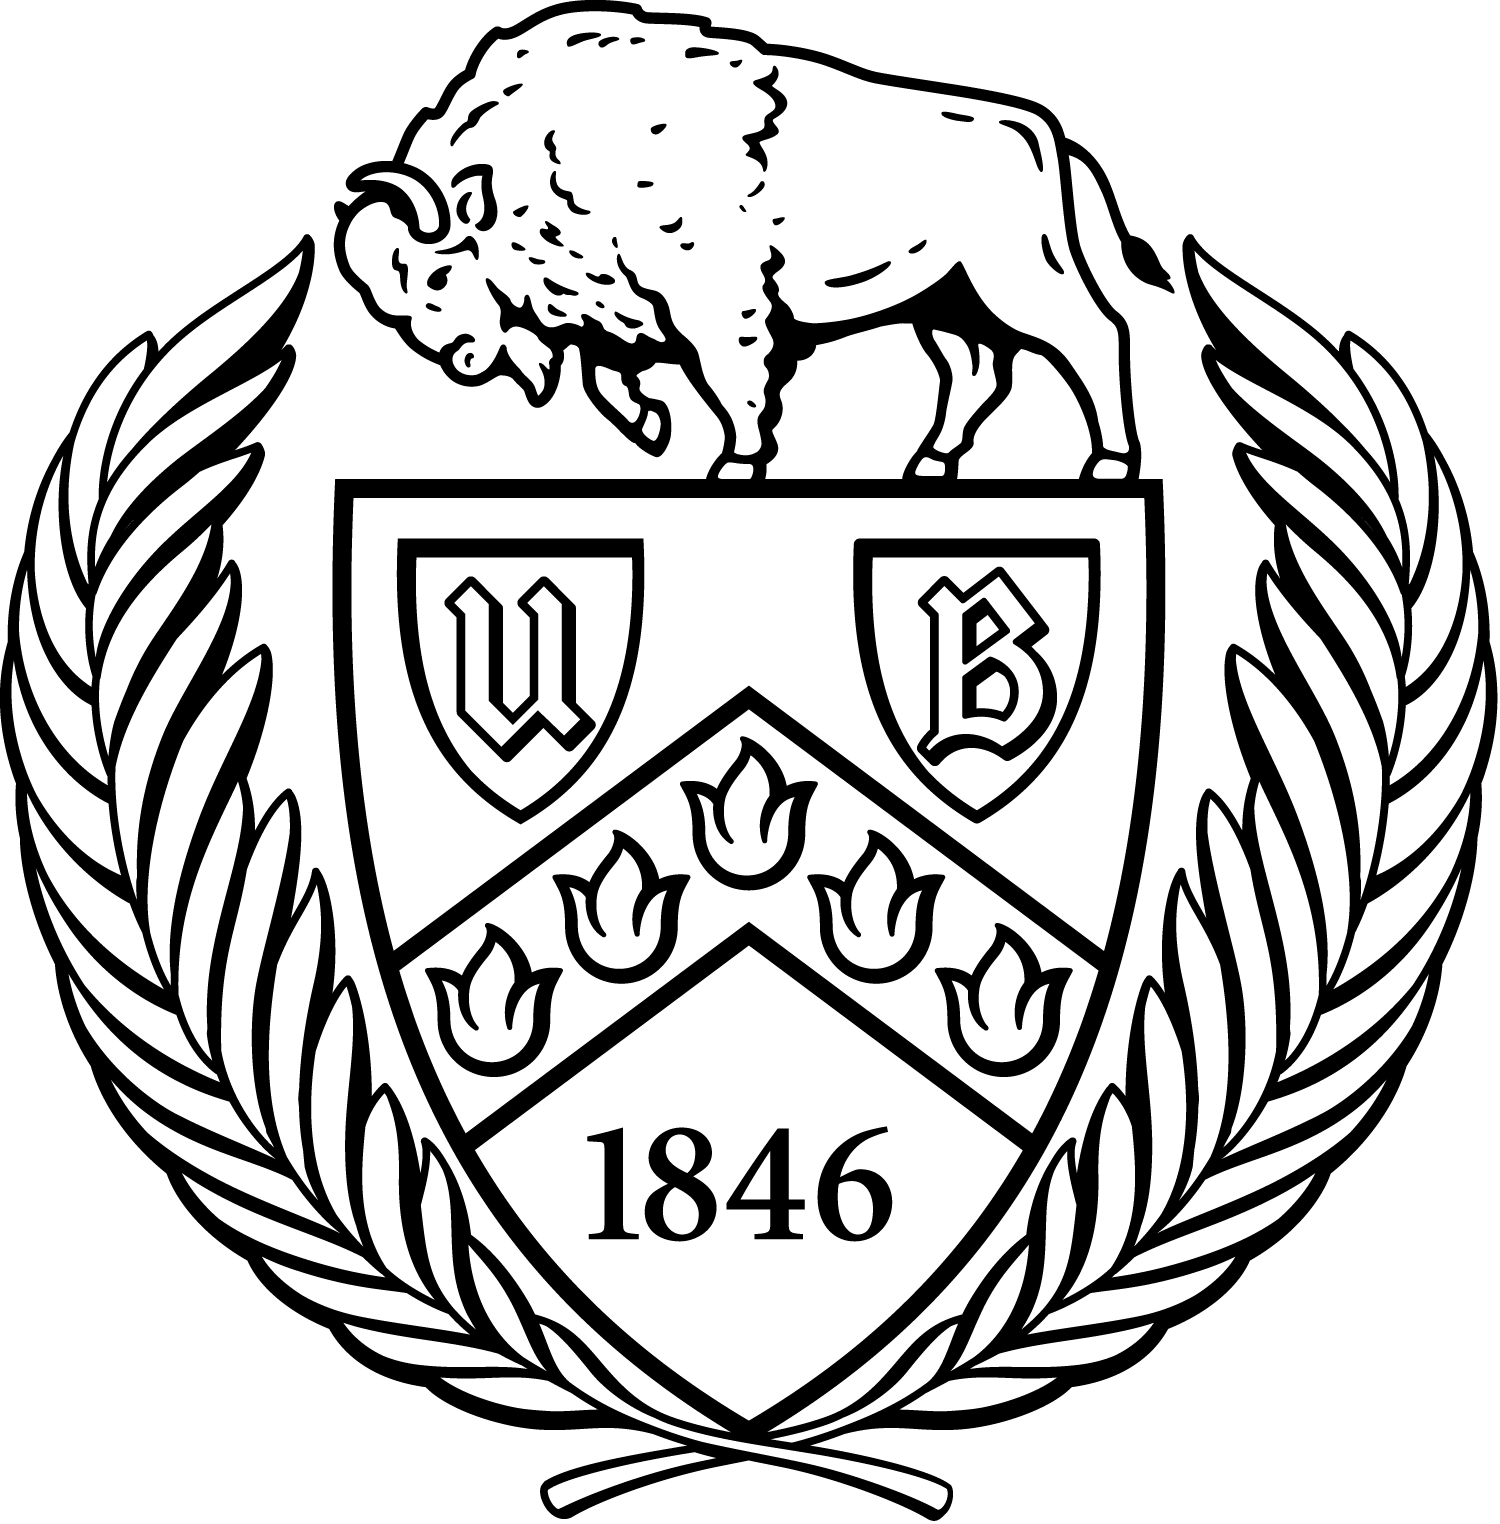
\includegraphics[
  width=6cm,
  height=6cm,
  keepaspectratio,
]{Crest_BW.png}\\[1cm] % Include a department/university logo - this will require the graphicx package
 
%----------------------------------------------------------------------------------------

\vfill % Fill the rest of the page with whitespace

\end{titlepage}

\title{\Large CSE 676: Deep Learning\\\Huge Assignment - 1}
\date{\today}
\author{Yash Narendra Saraf\\UB ID: 50290453\\\texttt{ysaraf@buffalo.edu}}
\maketitle
% //////////////////////////////////////////////////////////////////////////////////////////////////
% //////////////////////////////////////////////////////////////////////////////////////////////////
\section{Softmax [2 points]}

% //////////////////////////////////////////////////////////////////////////////////////////////////
\subsection{ [1 point] Prove that softmax is invariant to constant sifts in the input, i.e., for any
input vector x and a constant scalar c, the following holds: \\
$$ softmax(x) = softmax(x +c)  $$
 where $ softmax(x)_i \triangleq \dfrac{e^{x_i}}{\sum_{i_{'}}^{} e^{x_i^{'}}},$ and $ x +c $ means adding c to every dimension of x.}
 
 The definition of Softmax is - 
$$ softmax(x)_i \triangleq \dfrac{e^{x_i}}{\sum_{i_{'}}^{} e^{x_i^{'}}},$$

Now, we have to prove that even after constant shifts the output of the softmax won't change i.e.
$$ softmax(x) = softmax(x +c)  $$

So, replacing $x$ by $x+c$ in the original softmax equation, we have 
\begin{align*}
{softmax(x)_i &\triangleq \dfrac{e^{x_i}}{\sum_{i_{'}}^{} e^{x_i^{'}}}}\\
               &= \dfrac{e^{x_i + c}}{\sum_{i_{'}}^{} e^{x_i^{'}+c}}\\
               &= \dfrac{e^{c}*e^{x_i}}{e^{c} * \sum_{i_{'}}^{} e^{x_i^{'}}}\\
               &= \dfrac{e^{x_i}}{\sum_{i_{'}}^{} e^{x_i^{'}}}
\end{align*}

Hence Proved, softmax function is invariant to constant shifts. 

% //////////////////////////////////////////////////////////////////////////////////////////////////
\subsection{ [1 point] Let $z = W x + c$, where W and c are some matrix and vector, respectively.
Let \\
$$ J =  \sum_{i}^{}log  \, softmax(z_{i}) $$
 Calculate the derivatives of J w.r.t. W and c, respectively, i.e., calculate $ \frac{\partial J}{\partial W} $ and $ \frac{\partial J}{\partial c} $.}
 
 
For the calculation of $ \frac{\partial J}{\partial z} \ $, 

$$\frac{\partial J}{\partial z} =  -\frac{\partial}{\partial z} \ \sum_{i}^{}log  \, softmax(z_{i}) $$

Calculating the derivative by considering the derivative while doing calculations for Class i. 
This is necessary as when we use chain rule to calculate derivatives we will have different derivative for the class under considerations and all other classes. This is because of the derivative of the softmax function.  

$$\frac{\partial J}{\partial z} = -\frac{\partial}{\partial z}(log(softmax(z_i))) -\frac{\partial}{\partial z} \ \sum_{k\neq i}\, log(softmax(z_k))$$

$$\frac{\partial J}{\partial z} = -\Big(\frac{1}{(softmax(z_i))} \ \frac{\partial (softmax(z_i))}{\partial z}\Big) - \ \sum_{k\neq i}y_k \ \frac{1}{(softmax(z_k))} \frac{\partial (softmax(z_k))}{\partial z}$$


$$\frac{\partial J}{\partial z} = -(\ 1-(softmax(z_i))) + \ \sum_{k\neq i}\ (softmax(z_i))$$

$$\frac{\partial J}{\partial z} = -1 + (softmax(z_i)) + \ \sum_{k\neq i}(softmax(z_i))$$


$$\frac{\partial J(z)}{\partial z} = -1 + \ \Big(\sum_{k=1}^{N}1\Big) \ (softmax(z_i))$$


$$\frac{\partial J(z)}{\partial z} = -1 + \ N (softmax(z_i))$$ 

Now, we need to calculate the $ \frac{\partial J}{\partial W} $ and $ \frac{\partial J}{\partial c} $. This can be simply done by applying the chain rule as we know the values for $\frac{\partial J}{\partial z} $ and z. 

So, as  $z = W x + c$. 
We can write,  

$$\frac{\partial J}{\partial W}  = \frac{\partial J}{\partial z} \ \frac{\partial z}{\partial W}$$

$$\frac{\partial J}{\partial W}  = (-1 + \ N (softmax(z_i))) \ \frac{\partial z}{\partial W}$$

$$\frac{\partial J}{\partial W}  = (-1 + \ N (softmax(z_i))) \ x $$

and similarly for $ \frac{\partial J}{\partial c} $,


$$ \frac{\partial J}{\partial c}  = \frac{\partial J}{\partial z} \ \frac{\partial z}{\partial c}$$

$$\frac{\partial J}{\partial c}  = (-1 + \ N (softmax(z_i))) \ \frac{\partial z}{\partial c}$$

$$\frac{\partial J}{\partial c}  = (-1 + \ N (softmax(z_i))) \ $$


% //////////////////////////////////////////////////////////////////////////////////////////////////
% //////////////////////////////////////////////////////////////////////////////////////////////////
\section{Logistic Regression with Regularization [2 points]}
% //////////////////////////////////////////////////////////////////////////////////////////////////
\subsection{ [1 point] Let the data be $(x_i, y_i)_{i=1}^{N} $ where $ x_i \in R^{d} $ and $ y_i \in \{0,1\} $. Logistic regression is a binary classification model, with the probability of $y_i$ being 1 as:
$$ p(y_i;x_i,\theta) =  \sigma(\theta^Tx_i) \triangleq \dfrac{1}{1 + e^{-\theta^Tx_{i}}} $$
where $\theta$ is the model parameter. Assume we impose an L2 regularization term on the
parameter, defined as:
$$ R(\theta) = \dfrac{\lambda}{2}\theta^T\theta$$
with a positive constant $ \lambda$. Write out the final objective function for this logistic
regression with regularization model.
}

Let the given Hypothesis function be represented as - 

$$ h_\theta(x_i) = p(y_i = 1|x_i,\theta) =  \sigma(\theta^Tx_i) \triangleq \dfrac{1}{1 + e^{-\theta^Tx_{i}}} $$

and the Regularization term given is - 

$$ R(\theta) = \dfrac{\lambda}{2}\theta^T\theta$$

The above Hypothesis function gives the probability of predicting 1 for the given input. 

So, we can't use the Mean Square Error as the Loss function as it would not give convex function. So to solve this problem the loss function can be designed as following - 

$$ Cost(h_\theta(x_i), y_i) = -y_i\,log(h_\theta(x_i)) - (1-y_i)\,log(1-h_\theta(x_i))$$

Using the above cost function the Objective function can be designed as - 

$$J(\theta) = \frac{1}{N}\sum_{i=1}^{N}Cost(h_\theta(x_i), y_i) $$

The regularization term can be added to the equation, as the function of the regularizer is to make sure that the model does not overfit. It also makes sure that the value of weights remain as small as possible. There is a scaling factor involved with the regularization term to make sure that the regularizer does not hinder the model from learning just to minimize the weights. Let the parameter be $ \lambda $.

$$J(\theta) = \frac{1}{N}\sum_{i=1}^{N}Cost(h_\theta(x_i), y_i) \ + \  R(\theta)$$

The above function represents the Objective function for Logistic Regression Model. 

% //////////////////////////////////////////////////////////////////////////////////////////////////
\subsection{[1 point] If we use gradient descent to solve the model parameter. Derive the updating
rule for $\theta$ . Your answer should contain the derivation, not just the final answer}

Now, since we have obtained the Objective function, our goal is to use this function to find optimum weights for the model using Gradient Descent. The gradient descent algorithm tries to find the minima of the Objective function for optimization. Here, the minima can be easily found by derivating the cost function with respect to Weights i.e. $\theta$ and updating the weights. Derivating with respect to theta gives us the slope of the graph and we use the slope to travel to the minima of Objective function. 

So, we now have following equations - 


$$ h_\theta(x_i) = p(y_i = 1|x_i,\theta) =  \sigma(\theta^Tx_i) \triangleq \dfrac{1}{1 + e^{-\theta^Tx_{i}}} $$

$$ R(\theta) = \dfrac{\lambda}{2}\theta^T\theta$$

$$ Cost(h_\theta(x_i), y_i) = -y_i\,log(h_\theta(x_i)) - (1-y_i)\,log(1-h_\theta(x_i))$$

$$J(\theta) = \frac{1}{N}\sum_{i=1}^{N}Cost(h_\theta(x_i), y_i) \ + \  R(\theta)$$

To calculate gradient equation first let's just find derivative of Cost function. We can later substitute the same in the main equation for calculation of finding final gradient. 

$$ \frac{\partial Cost(h_\theta(x_i), y_i)}{\partial \theta_j} = -\Big(\frac{y_i}{h_\theta(x_i)} - \frac{1- y_i}{1 - h_\theta(x_i)}\Big) \ \frac{\partial \ h_\theta(x_i)}{\partial \ \theta_j} $$

Now, $h_\theta(x_i)$ is a sigmoid function and the derivative of sigmoid function is given by - 

$$ \frac{\partial Cost(h_\theta(x_i), y_i)}{\partial x} = h_\theta(x)(1-h_\theta(x))$$

So, using that updating our Gradient calculation, 

$$ \frac{\partial Cost(h_\theta(x_i), y_i)}{\partial \theta_j} = -\Big(\frac{y_i}{h_\theta(x_i)} - \frac{1- y_i}{1 - h_\theta(x_i)}\Big) \ h_\theta(x_i) \ (1-h_\theta(x_i)) \ \frac{\partial \ \theta^Tx_i}{\partial \ \theta_j} $$


$$ \frac{\partial Cost(h_\theta(x_i), y_i))}{\partial \theta_j} = -(y_i(1-h_\theta(x_i)) - (1-y_i)h_\theta(x_i)) \ x_{ij} $$

Here, $x_{ij}$ represents the $j^{th}$ weight when working with input $x_i$.    

$$ \frac{\partial Cost(h_\theta(x_i), y_i)}{\partial \theta_j} = -(y_i - h_\theta(x_i)) \ x_{ij} $$

Now, calculating the complete gradient equation using the above partial derivative. 

So, 

$$ \frac{\partial J(\theta)}{\partial \theta_j} = \frac{\partial}{\partial \theta_j} \Big(\frac{1}{N}\sum_{i=1}^{N}Cost(h_\theta(x_i), y_i) \ + \  R(\theta)\Big)$$


$$ \frac{\partial J(\theta)}{\partial \theta_j} =\frac{1}{N}\sum_{i=1}^{N} \frac{\partial}{\partial \theta_j} \ Cost(h_\theta(x_i), y_i) \ + \ \frac{\partial}{\partial \theta_j} R(\theta)$$


$$ \frac{\partial J(\theta)}{\partial \theta_j} =-\frac{1}{N}\sum_{i=1}^{N} (y_i - h_\theta(x_i)) \ x_{ij} \ + \ \frac{\partial}{\partial \theta_j} R(\theta)$$


$$ \frac{\partial J(\theta)}{\partial \theta_j} =-\frac{1}{N}\sum_{i=1}^{N} (y_i - h_\theta(x_i)) \ x_{ij} \ + \  \frac{\partial}{\partial \theta_j} R(\theta)$$

Now, calculating the derivative of Regularization term - 

$$ \frac{\partial}{\partial \theta_j} R(\theta) = \frac{\partial}{\partial \theta_j} \  \dfrac{\lambda}{2}\theta^T\theta $$ 

$$ \frac{\partial}{\partial \theta_j} R(\theta) = \dfrac{\lambda}{2} \ \frac{\partial}{\partial \theta_j} (\theta^T\theta) $$

$$ \frac{\partial}{\partial \theta_j} R(\theta) = \dfrac{\lambda}{2} \ (2 \ \theta_j) $$

$$ \frac{\partial}{\partial \theta_j} R(\theta) = \lambda \ \theta_j$$

Substituting, the same in the gradient equation. 

$$ \frac{\partial J(\theta)}{\partial \theta_j} =-\frac{1}{N}\sum_{i=1}^{N} (y_i - h_\theta(x_i)) \ x_{ij} \ + \  \lambda \ \theta_j$$

So, weight updation equation will look like, 

$$ \theta_j = \theta_j - \alpha \ \frac{\partial J(\theta)}{\partial \theta_j} $$

$$ \theta_j = \theta_j - \alpha \ (-\frac{1}{N}\sum_{i=1}^{N} (y_i - h_\theta(x_i)) \ x_{ij} \ + \  \lambda \ \theta_j) $$

$$ \theta_j = \theta_j - \alpha \ (\frac{1}{N}\sum_{i=1}^{N} (h_\theta(x_i)-y_i) \ x_{ij} \ + \  \lambda \ \theta_j) $$

The constants can be combined and the final equation looks like - 

$$ \theta_j = \theta_j\Big(1-\frac{\lambda}{N}\Big) - \alpha \ (\sum_{i=1}^{N} (h_\theta(x_i)-y_i) \ x_{ij}) $$

In, the above equation the $\lambda$ represents the regularization constant and $\alpha$ represents the learning rate. 

% //////////////////////////////////////////////////////////////////////////////////////////////////
% //////////////////////////////////////////////////////////////////////////////////////////////////
\section{Derivative of the Softmax Function [3 points]}

% //////////////////////////////////////////////////////////////////////////////////////////////////
\subsection{ [1 point] Define the loss function as 
$$ J(z) = -\sum_{k=1}^{K}y_k \, log \widetilde{y}_k $$ 
where  $\widetilde{y}_k = \dfrac{e^{z_k}}{\sum_{k^{'}}^{} e^{z_{k^{'}}}}$ , and $(y_1,.., y_K)$ is a known probability vector. Derive the  $ \frac{\partial J(z)}{\partial z} $.
Note  $z = (z_1,.., z_K)$ is a vector so  $ \frac{\partial J(z)}{\partial z} $ is in the form of a vector. Your answer should contain the derivation, not just the final answer.}

For the calculation of $ \frac{\partial J(z)}{\partial z} \ $, 

$$\frac{\partial J(z)}{\partial z} =  -\frac{\partial}{\partial z} \ \sum_{k=1}^{K}y_k \, log \widetilde{y}_k$$

Calculating the derivative by considering the derivative while doing calculations for Class i. 
This is necessary as when we use chain rule to calculate derivatives we will have different derivative for the class under considerations and all other classes. This is because of the derivative of the softmax function.  

$$\frac{\partial J(z)}{\partial z} = -\frac{\partial}{\partial z}(y_i \ log(\widetilde{y}_i)) -\frac{\partial}{\partial z} \ \sum_{k\neq i}y_k \, log \widetilde{y}_k$$

$$\frac{\partial J(z)}{\partial z} = -\Big(y_i \ \frac{1}{\widetilde{y}_i} \ \frac{\partial y_i}{\partial z}\Big) - \ \sum_{k\neq i}y_k \ \frac{1}{\widetilde{y}_k} \frac{\partial \widetilde{y}_k}{\partial z}$$



$$\frac{\partial J(z)}{\partial z} = -(y_i \ (1-\widetilde{y}_i)) + \ \sum_{k\neq i}y_k \ \widetilde{y}_i$$

$$\frac{\partial J(z)}{\partial z} = -y_i + y_i \ \widetilde{y}_i + \ \sum_{k\neq i}y_k \ \widetilde{y}_i$$


$$\frac{\partial J(z)}{\partial z} = -y_i + \ \Big(\sum_{k=1}^{N}y_k\Big) \ \widetilde{y}_i$$


$$\frac{\partial J(z)}{\partial z} = -y_i + \ \widetilde{y}_i$$

% //////////////////////////////////////////////////////////////////////////////////////////////////
\subsection{ [1 point] Assume the above softmax is the output layer of an FNN. Briefly explain
how the derivative is used in the back propagation algorithm.}

In the above answer, the J(z) function given is the Cross Entropy Loss function. So we found the derivative of the Cross Entropy with respect to the output of the final layer i.e. $ \frac{\partial J(z)}{\partial z} $ as $ z = W^T \ h + b$. So, now we know gradient for the last layer. 

Now, to when we update the value of each weights i.e. $W_{ij}$, where W is the node from Node i to Node j, we need the value of $ \frac{\partial J(z)}{\partial W_{ij}} $, so to calculate which there is a need to propagate the error calculated at the last layer, and use chain rule in Calculus to propagate the error backwards.. 

The $ \frac{\partial J(z)}{\partial W_{ij}} $ is calculated for each weight and all weights are updated for that particular iteration. 

The property of the loss function for softmax regression is that it only penalizes the output from the correct class. But when we calculate the gradient equation it can be seen that all the the incorrect classes also get affected based on how incorrect those classes are. 

% //////////////////////////////////////////////////////////////////////////////////////////////////
\subsection{ [1 points] Let $z = W^T h + b$, where W is a matrix, b and h are vectors. Use the
chain rule to calculate the gradient of W and b, i.e.,
$ \frac{\partial J}{\partial W} $ and $ \frac{\partial J}{\partial b} $, respectively}

In the first part we calculated the following, 

$$\frac{\partial J(z)}{\partial z} = -y_i + \ \widetilde{y}_i$$.

Now, if we need to calculate $ \frac{\partial J}{\partial W} $ and $ \frac{\partial J}{\partial b} $, we can simply use $z = W^T h + b$ and update based on this. 

So, 

$$ \frac{\partial J(z)}{\partial W}  =  \frac{\partial J(z)}{\partial z} \ \frac{\partial z}{\partial W} $$

$$ \frac{\partial J(z)}{\partial W}  =   (-y_i + \ \widetilde{y}_i)\ \frac{\partial z}{\partial W} $$

$$ \frac{\partial J(z)}{\partial W}  =   (-y_i + \ \widetilde{y}_i)\ \frac{\partial (W^T h + b)}{\partial W} $$


$$ \frac{\partial J(z)}{\partial W}  =   (-y_i + \ \widetilde{y}_i)\ \frac{\partial (W^T h + b)}{\partial W} $$


$$ \frac{\partial J(z)}{\partial W}  =   (-y_i + \ \widetilde{y}_i) \ h $$

and similarly for $ \frac{\partial J}{\partial b} $, 

$$ \frac{\partial J(z)}{\partial b}  =   (-y_i + \ \widetilde{y}_i)\ \frac{\partial (W^T h + b)}{\partial b} $$

$$ \frac{\partial J(z)}{\partial b}  =   (-y_i + \ \widetilde{y}_i) $$

% //////////////////////////////////////////////////////////////////////////////////////////////////
% //////////////////////////////////////////////////////////////////////////////////////////////////
\section{MNIST with FNN [3 points]}

% //////////////////////////////////////////////////////////////////////////////////////////////////
\subsection{[3 points] Design an FNN for MNIST classification. Implement the model and plot
two curves in one figure: i) training loss vs. training iterations; ii) test loss vs. training
iterations.\\
– You can use code from websites. However, you must reference (cite) the code in
your answer.\\
– Submission includes the plot of the two curves and the runnable code (with a
ReadMe file containing instructions on how to run the code).}

For this question code can be found in the submitted folder directory. 
The ReadMe has also been added for reference. \\
The name of the file is \textbf{Q4\_MNIST\_FNN.ipynb}\\
The code is written inside jupyter notebook. Also for reference the tensorflow tutorials slides were used along with this \href{https://github.com/aymericdamien/TensorFlow-Examples/blob/master/examples/3_NeuralNetworks/multilayer_perceptron.py}{GitHub Repository}. 




The result graphs for the code can be found below - \\
\begin{figure}[h]
\centering
\begin{minipage}{.5\textwidth}
  \centering
  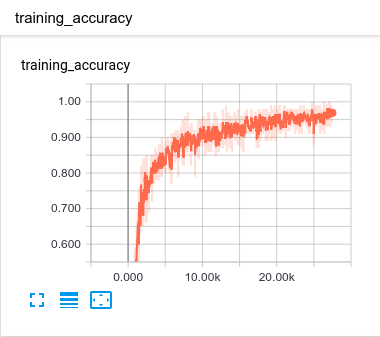
\includegraphics[width=.99\linewidth]{1.png}
  \captionof{}{Training Accuracy Graph}
\end{minipage}%
\begin{minipage}{.5\textwidth}
  \centering
  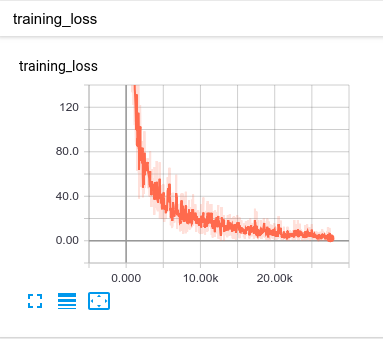
\includegraphics[width=.99\linewidth]{2.png}
  \captionof{}{Training Cost Graph}
\end{minipage}
\end{figure}

\begin{figure}[h]
\centering
\begin{minipage}{.5\textwidth}
  \centering
  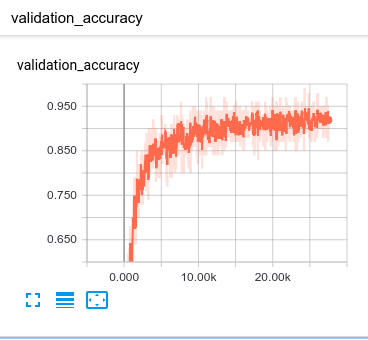
\includegraphics[width=.99\linewidth]{3.png}
  \captionof{}{Validation Accuracy Graph}
\end{minipage}%
\begin{minipage}{.5\textwidth}
  \centering
  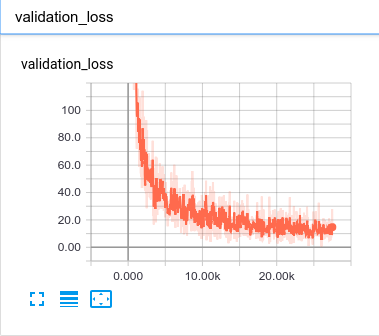
\includegraphics[width=.99\linewidth]{4.png}
  \captionof{}{Validation Cost Graph}
\end{minipage}
\end{figure}
    
\end{document} to your LaTeX file where you want your
% title page.
%
%%%%%%%%%%%%%%%%%%%%%%%%%%%%%%%%%%%%%%%%%
%\title{Title page with logo}
%----------------------------------------------------------------------------------------
%	PACKAGES AND OTHER DOCUMENT CONFIGURATIONS
%----------------------------------------------------------------------------------------

\documentclass[12]{article}
\usepackage[letterpaper, margin=0.5in, top=0.5in]{geometry}
\usepackage{enumitem}
\usepackage{mathtools}
\usepackage{amssymb}
% \usepackage{amsmath}
\usepackage{listings}
\usepackage{color}
\usepackage{cancel}
\usepackage{paracol}
\usepackage{dcolumn}
\usepackage[english]{babel}
\usepackage[utf8x]{inputenc}
\usepackage{amsmath}
\usepackage{graphicx}
\usepackage[colorinlistoftodos]{todonotes}
\usepackage{hyperref}

\renewcommand{\thesection}{Q\arabic{section}}
\renewcommand{\thesubsection}{(\arabic{subsection})}
\newcommand{\equno}[1]{\ensuremath{\stepcounter{equation}\tag{\theequation}\label{#1}}}
\newcommand{\bref}[1]{\textbf{\texttt{#1}}}

\definecolor{codeGray}{rgb}{0.8,0.8,0.8}
\lstdefinestyle{codeBlock}{
	backgroundcolor=\color{codeGray},
	frame=single,
	tabsize=2,
	captionpos=b
}
\hypersetup{
    colorlinks=true,
    linkcolor=blue,
    filecolor=magenta,      
    urlcolor=cyan,
}
\lstset{style=codeBlock}

\begin{document}

\begin{titlepage}

\newcommand{\HRule}{\rule{\linewidth}{0.5mm}} % Defines a new command for the horizontal lines, change thickness here

\center % Center everything on the page
 
%----------------------------------------------------------------------------------------
%	HEADING SECTIONS
%----------------------------------------------------------------------------------------
\vspace*{150px}
\textsc{\LARGE University at Buffalo, \\The State University of New York}\\[1.5cm] % Name of your university/college
\textsc{\large CSE 676}\\[0.5cm] % Major heading such as course name
\textsc{\large Deep Learning}\\[0.5cm] % Minor heading such as course title

%----------------------------------------------------------------------------------------
%	TITLE SECTION
%----------------------------------------------------------------------------------------

\HRule \\[0.4cm]
{ \LARGE \bfseries Assignment - 1}\\[0.4cm] % Title of your document
\HRule \\[1.5cm]
 
%----------------------------------------------------------------------------------------
%	AUTHOR SECTION
%----------------------------------------------------------------------------------------

\begin{center}
% \emph{Author:}\\
\Large Yash Narendra Saraf (50290453)\\
\end{center}


% If you don't want a supervisor, uncomment the two lines below and remove the section above
%\Large \emph{Author:}\\
%John \textsc{Smith}\\[3cm] % Your name

%----------------------------------------------------------------------------------------
%	DATE SECTION
%----------------------------------------------------------------------------------------
% Date, change the \today to a set date if you want to be precise

%----------------------------------------------------------------------------------------
%	LOGO SECTION
%----------------------------------------------------------------------------------------

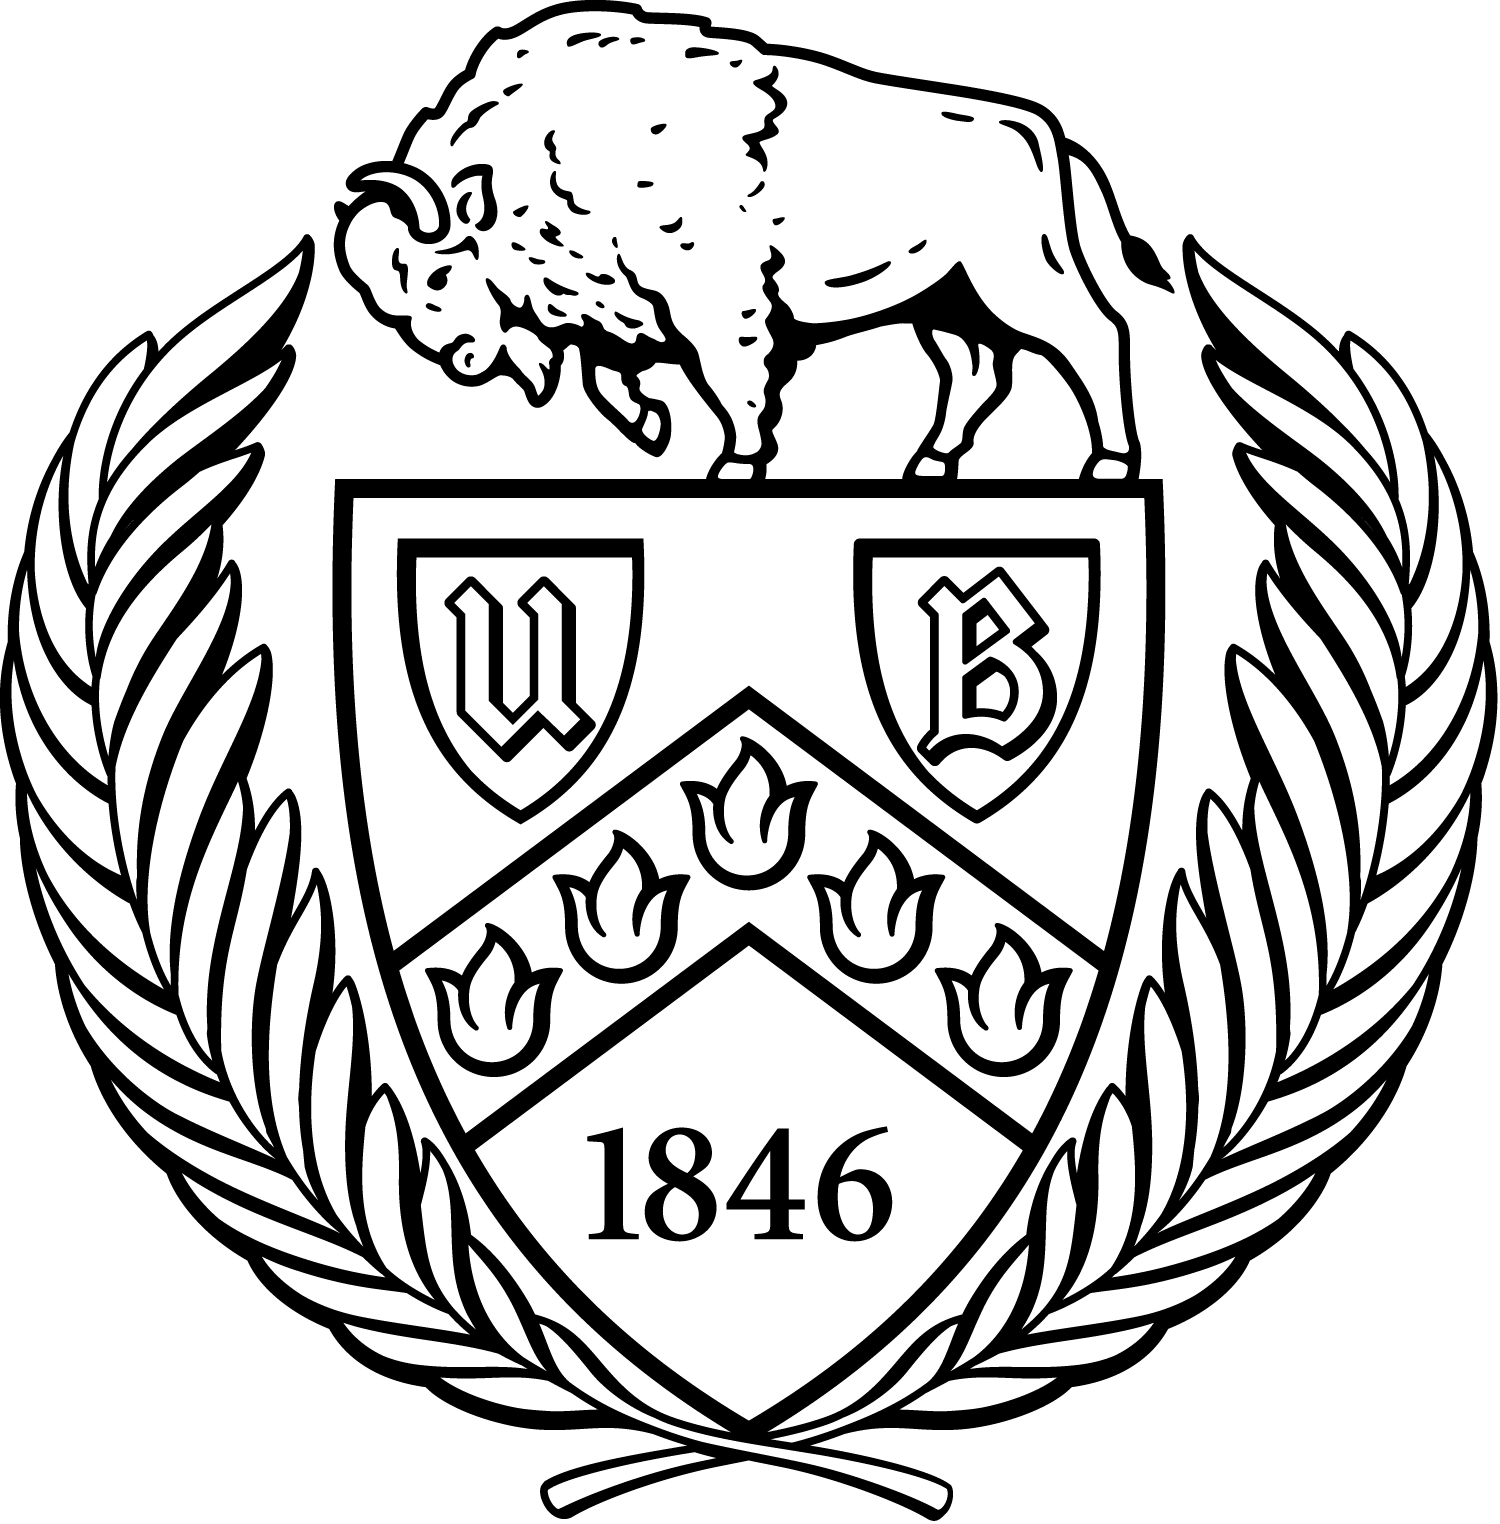
\includegraphics[
  width=6cm,
  height=6cm,
  keepaspectratio,
]{Crest_BW.png}\\[1cm] % Include a department/university logo - this will require the graphicx package
 
%----------------------------------------------------------------------------------------

\vfill % Fill the rest of the page with whitespace

\end{titlepage}

\title{\Large CSE 676: Deep Learning\\\Huge Assignment - 1}
\date{\today}
\author{Yash Narendra Saraf\\UB ID: 50290453\\\texttt{ysaraf@buffalo.edu}}
\maketitle
% //////////////////////////////////////////////////////////////////////////////////////////////////
% //////////////////////////////////////////////////////////////////////////////////////////////////
\section{Softmax [2 points]}

% //////////////////////////////////////////////////////////////////////////////////////////////////
\subsection{ [1 point] Prove that softmax is invariant to constant sifts in the input, i.e., for any
input vector x and a constant scalar c, the following holds: \\
$$ softmax(x) = softmax(x +c)  $$
 where $ softmax(x)_i \triangleq \dfrac{e^{x_i}}{\sum_{i_{'}}^{} e^{x_i^{'}}},$ and $ x +c $ means adding c to every dimension of x.}
 
 The definition of Softmax is - 
$$ softmax(x)_i \triangleq \dfrac{e^{x_i}}{\sum_{i_{'}}^{} e^{x_i^{'}}},$$

Now, we have to prove that even after constant shifts the output of the softmax won't change i.e.
$$ softmax(x) = softmax(x +c)  $$

So, replacing $x$ by $x+c$ in the original softmax equation, we have 
\begin{align*}
{softmax(x)_i &\triangleq \dfrac{e^{x_i}}{\sum_{i_{'}}^{} e^{x_i^{'}}}}\\
               &= \dfrac{e^{x_i + c}}{\sum_{i_{'}}^{} e^{x_i^{'}+c}}\\
               &= \dfrac{e^{c}*e^{x_i}}{e^{c} * \sum_{i_{'}}^{} e^{x_i^{'}}}\\
               &= \dfrac{e^{x_i}}{\sum_{i_{'}}^{} e^{x_i^{'}}}
\end{align*}

Hence Proved, softmax function is invariant to constant shifts. 

% //////////////////////////////////////////////////////////////////////////////////////////////////
\subsection{ [1 point] Let $z = W x + c$, where W and c are some matrix and vector, respectively.
Let \\
$$ J =  \sum_{i}^{}log  \, softmax(z_{i}) $$
 Calculate the derivatives of J w.r.t. W and c, respectively, i.e., calculate $ \frac{\partial J}{\partial W} $ and $ \frac{\partial J}{\partial c} $.}
 
 
For the calculation of $ \frac{\partial J}{\partial z} \ $, 

$$\frac{\partial J}{\partial z} =  -\frac{\partial}{\partial z} \ \sum_{i}^{}log  \, softmax(z_{i}) $$

Calculating the derivative by considering the derivative while doing calculations for Class i. 
This is necessary as when we use chain rule to calculate derivatives we will have different derivative for the class under considerations and all other classes. This is because of the derivative of the softmax function.  

$$\frac{\partial J}{\partial z} = -\frac{\partial}{\partial z}(log(softmax(z_i))) -\frac{\partial}{\partial z} \ \sum_{k\neq i}\, log(softmax(z_k))$$

$$\frac{\partial J}{\partial z} = -\Big(\frac{1}{(softmax(z_i))} \ \frac{\partial (softmax(z_i))}{\partial z}\Big) - \ \sum_{k\neq i}y_k \ \frac{1}{(softmax(z_k))} \frac{\partial (softmax(z_k))}{\partial z}$$


$$\frac{\partial J}{\partial z} = -(\ 1-(softmax(z_i))) + \ \sum_{k\neq i}\ (softmax(z_i))$$

$$\frac{\partial J}{\partial z} = -1 + (softmax(z_i)) + \ \sum_{k\neq i}(softmax(z_i))$$


$$\frac{\partial J(z)}{\partial z} = -1 + \ \Big(\sum_{k=1}^{N}1\Big) \ (softmax(z_i))$$


$$\frac{\partial J(z)}{\partial z} = -1 + \ N (softmax(z_i))$$ 

Now, we need to calculate the $ \frac{\partial J}{\partial W} $ and $ \frac{\partial J}{\partial c} $. This can be simply done by applying the chain rule as we know the values for $\frac{\partial J}{\partial z} $ and z. 

So, as  $z = W x + c$. 
We can write,  

$$\frac{\partial J}{\partial W}  = \frac{\partial J}{\partial z} \ \frac{\partial z}{\partial W}$$

$$\frac{\partial J}{\partial W}  = (-1 + \ N (softmax(z_i))) \ \frac{\partial z}{\partial W}$$

$$\frac{\partial J}{\partial W}  = (-1 + \ N (softmax(z_i))) \ x $$

and similarly for $ \frac{\partial J}{\partial c} $,


$$ \frac{\partial J}{\partial c}  = \frac{\partial J}{\partial z} \ \frac{\partial z}{\partial c}$$

$$\frac{\partial J}{\partial c}  = (-1 + \ N (softmax(z_i))) \ \frac{\partial z}{\partial c}$$

$$\frac{\partial J}{\partial c}  = (-1 + \ N (softmax(z_i))) \ $$


% //////////////////////////////////////////////////////////////////////////////////////////////////
% //////////////////////////////////////////////////////////////////////////////////////////////////
\section{Logistic Regression with Regularization [2 points]}
% //////////////////////////////////////////////////////////////////////////////////////////////////
\subsection{ [1 point] Let the data be $(x_i, y_i)_{i=1}^{N} $ where $ x_i \in R^{d} $ and $ y_i \in \{0,1\} $. Logistic regression is a binary classification model, with the probability of $y_i$ being 1 as:
$$ p(y_i;x_i,\theta) =  \sigma(\theta^Tx_i) \triangleq \dfrac{1}{1 + e^{-\theta^Tx_{i}}} $$
where $\theta$ is the model parameter. Assume we impose an L2 regularization term on the
parameter, defined as:
$$ R(\theta) = \dfrac{\lambda}{2}\theta^T\theta$$
with a positive constant $ \lambda$. Write out the final objective function for this logistic
regression with regularization model.
}

Let the given Hypothesis function be represented as - 

$$ h_\theta(x_i) = p(y_i = 1|x_i,\theta) =  \sigma(\theta^Tx_i) \triangleq \dfrac{1}{1 + e^{-\theta^Tx_{i}}} $$

and the Regularization term given is - 

$$ R(\theta) = \dfrac{\lambda}{2}\theta^T\theta$$

The above Hypothesis function gives the probability of predicting 1 for the given input. 

So, we can't use the Mean Square Error as the Loss function as it would not give convex function. So to solve this problem the loss function can be designed as following - 

$$ Cost(h_\theta(x_i), y_i) = -y_i\,log(h_\theta(x_i)) - (1-y_i)\,log(1-h_\theta(x_i))$$

Using the above cost function the Objective function can be designed as - 

$$J(\theta) = \frac{1}{N}\sum_{i=1}^{N}Cost(h_\theta(x_i), y_i) $$

The regularization term can be added to the equation, as the function of the regularizer is to make sure that the model does not overfit. It also makes sure that the value of weights remain as small as possible. There is a scaling factor involved with the regularization term to make sure that the regularizer does not hinder the model from learning just to minimize the weights. Let the parameter be $ \lambda $.

$$J(\theta) = \frac{1}{N}\sum_{i=1}^{N}Cost(h_\theta(x_i), y_i) \ + \  R(\theta)$$

The above function represents the Objective function for Logistic Regression Model. 

% //////////////////////////////////////////////////////////////////////////////////////////////////
\subsection{[1 point] If we use gradient descent to solve the model parameter. Derive the updating
rule for $\theta$ . Your answer should contain the derivation, not just the final answer}

Now, since we have obtained the Objective function, our goal is to use this function to find optimum weights for the model using Gradient Descent. The gradient descent algorithm tries to find the minima of the Objective function for optimization. Here, the minima can be easily found by derivating the cost function with respect to Weights i.e. $\theta$ and updating the weights. Derivating with respect to theta gives us the slope of the graph and we use the slope to travel to the minima of Objective function. 

So, we now have following equations - 


$$ h_\theta(x_i) = p(y_i = 1|x_i,\theta) =  \sigma(\theta^Tx_i) \triangleq \dfrac{1}{1 + e^{-\theta^Tx_{i}}} $$

$$ R(\theta) = \dfrac{\lambda}{2}\theta^T\theta$$

$$ Cost(h_\theta(x_i), y_i) = -y_i\,log(h_\theta(x_i)) - (1-y_i)\,log(1-h_\theta(x_i))$$

$$J(\theta) = \frac{1}{N}\sum_{i=1}^{N}Cost(h_\theta(x_i), y_i) \ + \  R(\theta)$$

To calculate gradient equation first let's just find derivative of Cost function. We can later substitute the same in the main equation for calculation of finding final gradient. 

$$ \frac{\partial Cost(h_\theta(x_i), y_i)}{\partial \theta_j} = -\Big(\frac{y_i}{h_\theta(x_i)} - \frac{1- y_i}{1 - h_\theta(x_i)}\Big) \ \frac{\partial \ h_\theta(x_i)}{\partial \ \theta_j} $$

Now, $h_\theta(x_i)$ is a sigmoid function and the derivative of sigmoid function is given by - 

$$ \frac{\partial Cost(h_\theta(x_i), y_i)}{\partial x} = h_\theta(x)(1-h_\theta(x))$$

So, using that updating our Gradient calculation, 

$$ \frac{\partial Cost(h_\theta(x_i), y_i)}{\partial \theta_j} = -\Big(\frac{y_i}{h_\theta(x_i)} - \frac{1- y_i}{1 - h_\theta(x_i)}\Big) \ h_\theta(x_i) \ (1-h_\theta(x_i)) \ \frac{\partial \ \theta^Tx_i}{\partial \ \theta_j} $$


$$ \frac{\partial Cost(h_\theta(x_i), y_i))}{\partial \theta_j} = -(y_i(1-h_\theta(x_i)) - (1-y_i)h_\theta(x_i)) \ x_{ij} $$

Here, $x_{ij}$ represents the $j^{th}$ weight when working with input $x_i$.    

$$ \frac{\partial Cost(h_\theta(x_i), y_i)}{\partial \theta_j} = -(y_i - h_\theta(x_i)) \ x_{ij} $$

Now, calculating the complete gradient equation using the above partial derivative. 

So, 

$$ \frac{\partial J(\theta)}{\partial \theta_j} = \frac{\partial}{\partial \theta_j} \Big(\frac{1}{N}\sum_{i=1}^{N}Cost(h_\theta(x_i), y_i) \ + \  R(\theta)\Big)$$


$$ \frac{\partial J(\theta)}{\partial \theta_j} =\frac{1}{N}\sum_{i=1}^{N} \frac{\partial}{\partial \theta_j} \ Cost(h_\theta(x_i), y_i) \ + \ \frac{\partial}{\partial \theta_j} R(\theta)$$


$$ \frac{\partial J(\theta)}{\partial \theta_j} =-\frac{1}{N}\sum_{i=1}^{N} (y_i - h_\theta(x_i)) \ x_{ij} \ + \ \frac{\partial}{\partial \theta_j} R(\theta)$$


$$ \frac{\partial J(\theta)}{\partial \theta_j} =-\frac{1}{N}\sum_{i=1}^{N} (y_i - h_\theta(x_i)) \ x_{ij} \ + \  \frac{\partial}{\partial \theta_j} R(\theta)$$

Now, calculating the derivative of Regularization term - 

$$ \frac{\partial}{\partial \theta_j} R(\theta) = \frac{\partial}{\partial \theta_j} \  \dfrac{\lambda}{2}\theta^T\theta $$ 

$$ \frac{\partial}{\partial \theta_j} R(\theta) = \dfrac{\lambda}{2} \ \frac{\partial}{\partial \theta_j} (\theta^T\theta) $$

$$ \frac{\partial}{\partial \theta_j} R(\theta) = \dfrac{\lambda}{2} \ (2 \ \theta_j) $$

$$ \frac{\partial}{\partial \theta_j} R(\theta) = \lambda \ \theta_j$$

Substituting, the same in the gradient equation. 

$$ \frac{\partial J(\theta)}{\partial \theta_j} =-\frac{1}{N}\sum_{i=1}^{N} (y_i - h_\theta(x_i)) \ x_{ij} \ + \  \lambda \ \theta_j$$

So, weight updation equation will look like, 

$$ \theta_j = \theta_j - \alpha \ \frac{\partial J(\theta)}{\partial \theta_j} $$

$$ \theta_j = \theta_j - \alpha \ (-\frac{1}{N}\sum_{i=1}^{N} (y_i - h_\theta(x_i)) \ x_{ij} \ + \  \lambda \ \theta_j) $$

$$ \theta_j = \theta_j - \alpha \ (\frac{1}{N}\sum_{i=1}^{N} (h_\theta(x_i)-y_i) \ x_{ij} \ + \  \lambda \ \theta_j) $$

The constants can be combined and the final equation looks like - 

$$ \theta_j = \theta_j\Big(1-\frac{\lambda}{N}\Big) - \alpha \ (\sum_{i=1}^{N} (h_\theta(x_i)-y_i) \ x_{ij}) $$

In, the above equation the $\lambda$ represents the regularization constant and $\alpha$ represents the learning rate. 

% //////////////////////////////////////////////////////////////////////////////////////////////////
% //////////////////////////////////////////////////////////////////////////////////////////////////
\section{Derivative of the Softmax Function [3 points]}

% //////////////////////////////////////////////////////////////////////////////////////////////////
\subsection{ [1 point] Define the loss function as 
$$ J(z) = -\sum_{k=1}^{K}y_k \, log \widetilde{y}_k $$ 
where  $\widetilde{y}_k = \dfrac{e^{z_k}}{\sum_{k^{'}}^{} e^{z_{k^{'}}}}$ , and $(y_1,.., y_K)$ is a known probability vector. Derive the  $ \frac{\partial J(z)}{\partial z} $.
Note  $z = (z_1,.., z_K)$ is a vector so  $ \frac{\partial J(z)}{\partial z} $ is in the form of a vector. Your answer should contain the derivation, not just the final answer.}

For the calculation of $ \frac{\partial J(z)}{\partial z} \ $, 

$$\frac{\partial J(z)}{\partial z} =  -\frac{\partial}{\partial z} \ \sum_{k=1}^{K}y_k \, log \widetilde{y}_k$$

Calculating the derivative by considering the derivative while doing calculations for Class i. 
This is necessary as when we use chain rule to calculate derivatives we will have different derivative for the class under considerations and all other classes. This is because of the derivative of the softmax function.  

$$\frac{\partial J(z)}{\partial z} = -\frac{\partial}{\partial z}(y_i \ log(\widetilde{y}_i)) -\frac{\partial}{\partial z} \ \sum_{k\neq i}y_k \, log \widetilde{y}_k$$

$$\frac{\partial J(z)}{\partial z} = -\Big(y_i \ \frac{1}{\widetilde{y}_i} \ \frac{\partial y_i}{\partial z}\Big) - \ \sum_{k\neq i}y_k \ \frac{1}{\widetilde{y}_k} \frac{\partial \widetilde{y}_k}{\partial z}$$



$$\frac{\partial J(z)}{\partial z} = -(y_i \ (1-\widetilde{y}_i)) + \ \sum_{k\neq i}y_k \ \widetilde{y}_i$$

$$\frac{\partial J(z)}{\partial z} = -y_i + y_i \ \widetilde{y}_i + \ \sum_{k\neq i}y_k \ \widetilde{y}_i$$


$$\frac{\partial J(z)}{\partial z} = -y_i + \ \Big(\sum_{k=1}^{N}y_k\Big) \ \widetilde{y}_i$$


$$\frac{\partial J(z)}{\partial z} = -y_i + \ \widetilde{y}_i$$

% //////////////////////////////////////////////////////////////////////////////////////////////////
\subsection{ [1 point] Assume the above softmax is the output layer of an FNN. Briefly explain
how the derivative is used in the back propagation algorithm.}

In the above answer, the J(z) function given is the Cross Entropy Loss function. So we found the derivative of the Cross Entropy with respect to the output of the final layer i.e. $ \frac{\partial J(z)}{\partial z} $ as $ z = W^T \ h + b$. So, now we know gradient for the last layer. 

Now, to when we update the value of each weights i.e. $W_{ij}$, where W is the node from Node i to Node j, we need the value of $ \frac{\partial J(z)}{\partial W_{ij}} $, so to calculate which there is a need to propagate the error calculated at the last layer, and use chain rule in Calculus to propagate the error backwards.. 

The $ \frac{\partial J(z)}{\partial W_{ij}} $ is calculated for each weight and all weights are updated for that particular iteration. 

The property of the loss function for softmax regression is that it only penalizes the output from the correct class. But when we calculate the gradient equation it can be seen that all the the incorrect classes also get affected based on how incorrect those classes are. 

% //////////////////////////////////////////////////////////////////////////////////////////////////
\subsection{ [1 points] Let $z = W^T h + b$, where W is a matrix, b and h are vectors. Use the
chain rule to calculate the gradient of W and b, i.e.,
$ \frac{\partial J}{\partial W} $ and $ \frac{\partial J}{\partial b} $, respectively}

In the first part we calculated the following, 

$$\frac{\partial J(z)}{\partial z} = -y_i + \ \widetilde{y}_i$$.

Now, if we need to calculate $ \frac{\partial J}{\partial W} $ and $ \frac{\partial J}{\partial b} $, we can simply use $z = W^T h + b$ and update based on this. 

So, 

$$ \frac{\partial J(z)}{\partial W}  =  \frac{\partial J(z)}{\partial z} \ \frac{\partial z}{\partial W} $$

$$ \frac{\partial J(z)}{\partial W}  =   (-y_i + \ \widetilde{y}_i)\ \frac{\partial z}{\partial W} $$

$$ \frac{\partial J(z)}{\partial W}  =   (-y_i + \ \widetilde{y}_i)\ \frac{\partial (W^T h + b)}{\partial W} $$


$$ \frac{\partial J(z)}{\partial W}  =   (-y_i + \ \widetilde{y}_i)\ \frac{\partial (W^T h + b)}{\partial W} $$


$$ \frac{\partial J(z)}{\partial W}  =   (-y_i + \ \widetilde{y}_i) \ h $$

and similarly for $ \frac{\partial J}{\partial b} $, 

$$ \frac{\partial J(z)}{\partial b}  =   (-y_i + \ \widetilde{y}_i)\ \frac{\partial (W^T h + b)}{\partial b} $$

$$ \frac{\partial J(z)}{\partial b}  =   (-y_i + \ \widetilde{y}_i) $$

% //////////////////////////////////////////////////////////////////////////////////////////////////
% //////////////////////////////////////////////////////////////////////////////////////////////////
\section{MNIST with FNN [3 points]}

% //////////////////////////////////////////////////////////////////////////////////////////////////
\subsection{[3 points] Design an FNN for MNIST classification. Implement the model and plot
two curves in one figure: i) training loss vs. training iterations; ii) test loss vs. training
iterations.\\
– You can use code from websites. However, you must reference (cite) the code in
your answer.\\
– Submission includes the plot of the two curves and the runnable code (with a
ReadMe file containing instructions on how to run the code).}

For this question code can be found in the submitted folder directory. 
The ReadMe has also been added for reference. \\
The name of the file is \textbf{Q4\_MNIST\_FNN.ipynb}\\
The code is written inside jupyter notebook. Also for reference the tensorflow tutorials slides were used along with this \href{https://github.com/aymericdamien/TensorFlow-Examples/blob/master/examples/3_NeuralNetworks/multilayer_perceptron.py}{GitHub Repository}. 




The result graphs for the code can be found below - \\
\begin{figure}[h]
\centering
\begin{minipage}{.5\textwidth}
  \centering
  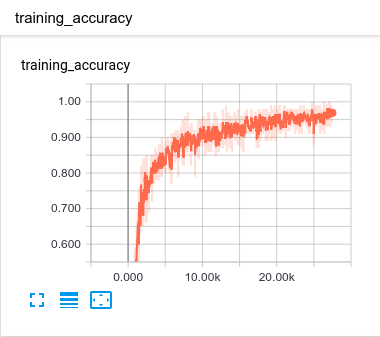
\includegraphics[width=.99\linewidth]{1.png}
  \captionof{}{Training Accuracy Graph}
\end{minipage}%
\begin{minipage}{.5\textwidth}
  \centering
  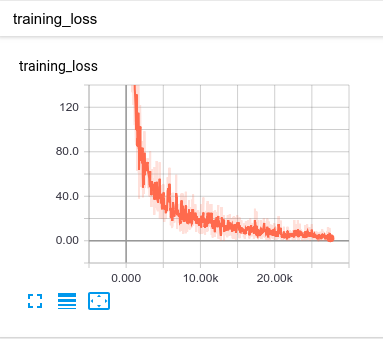
\includegraphics[width=.99\linewidth]{2.png}
  \captionof{}{Training Cost Graph}
\end{minipage}
\end{figure}

\begin{figure}[h]
\centering
\begin{minipage}{.5\textwidth}
  \centering
  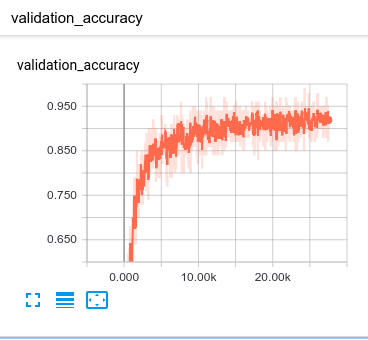
\includegraphics[width=.99\linewidth]{3.png}
  \captionof{}{Validation Accuracy Graph}
\end{minipage}%
\begin{minipage}{.5\textwidth}
  \centering
  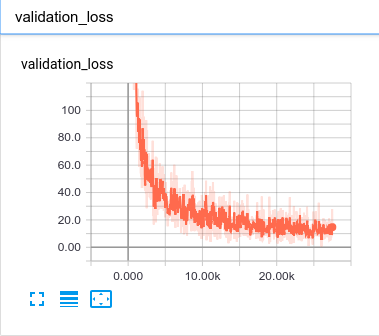
\includegraphics[width=.99\linewidth]{4.png}
  \captionof{}{Validation Cost Graph}
\end{minipage}
\end{figure}
    
\end{document} to your LaTeX file where you want your
% title page.
%
%%%%%%%%%%%%%%%%%%%%%%%%%%%%%%%%%%%%%%%%%
%\title{Title page with logo}
%----------------------------------------------------------------------------------------
%	PACKAGES AND OTHER DOCUMENT CONFIGURATIONS
%----------------------------------------------------------------------------------------

\documentclass[12]{article}
\usepackage[letterpaper, margin=0.5in, top=0.5in]{geometry}
\usepackage{enumitem}
\usepackage{mathtools}
\usepackage{amssymb}
% \usepackage{amsmath}
\usepackage{listings}
\usepackage{color}
\usepackage{cancel}
\usepackage{paracol}
\usepackage{dcolumn}
\usepackage[english]{babel}
\usepackage[utf8x]{inputenc}
\usepackage{amsmath}
\usepackage{graphicx}
\usepackage[colorinlistoftodos]{todonotes}
\usepackage{hyperref}

\renewcommand{\thesection}{Q\arabic{section}}
\renewcommand{\thesubsection}{(\arabic{subsection})}
\newcommand{\equno}[1]{\ensuremath{\stepcounter{equation}\tag{\theequation}\label{#1}}}
\newcommand{\bref}[1]{\textbf{\texttt{#1}}}

\definecolor{codeGray}{rgb}{0.8,0.8,0.8}
\lstdefinestyle{codeBlock}{
	backgroundcolor=\color{codeGray},
	frame=single,
	tabsize=2,
	captionpos=b
}
\hypersetup{
    colorlinks=true,
    linkcolor=blue,
    filecolor=magenta,      
    urlcolor=cyan,
}
\lstset{style=codeBlock}

\begin{document}

\begin{titlepage}

\newcommand{\HRule}{\rule{\linewidth}{0.5mm}} % Defines a new command for the horizontal lines, change thickness here

\center % Center everything on the page
 
%----------------------------------------------------------------------------------------
%	HEADING SECTIONS
%----------------------------------------------------------------------------------------
\vspace*{150px}
\textsc{\LARGE University at Buffalo, \\The State University of New York}\\[1.5cm] % Name of your university/college
\textsc{\large CSE 676}\\[0.5cm] % Major heading such as course name
\textsc{\large Deep Learning}\\[0.5cm] % Minor heading such as course title

%----------------------------------------------------------------------------------------
%	TITLE SECTION
%----------------------------------------------------------------------------------------

\HRule \\[0.4cm]
{ \LARGE \bfseries Assignment - 1}\\[0.4cm] % Title of your document
\HRule \\[1.5cm]
 
%----------------------------------------------------------------------------------------
%	AUTHOR SECTION
%----------------------------------------------------------------------------------------

\begin{center}
% \emph{Author:}\\
\Large Yash Narendra Saraf (50290453)\\
\end{center}


% If you don't want a supervisor, uncomment the two lines below and remove the section above
%\Large \emph{Author:}\\
%John \textsc{Smith}\\[3cm] % Your name

%----------------------------------------------------------------------------------------
%	DATE SECTION
%----------------------------------------------------------------------------------------
% Date, change the \today to a set date if you want to be precise

%----------------------------------------------------------------------------------------
%	LOGO SECTION
%----------------------------------------------------------------------------------------

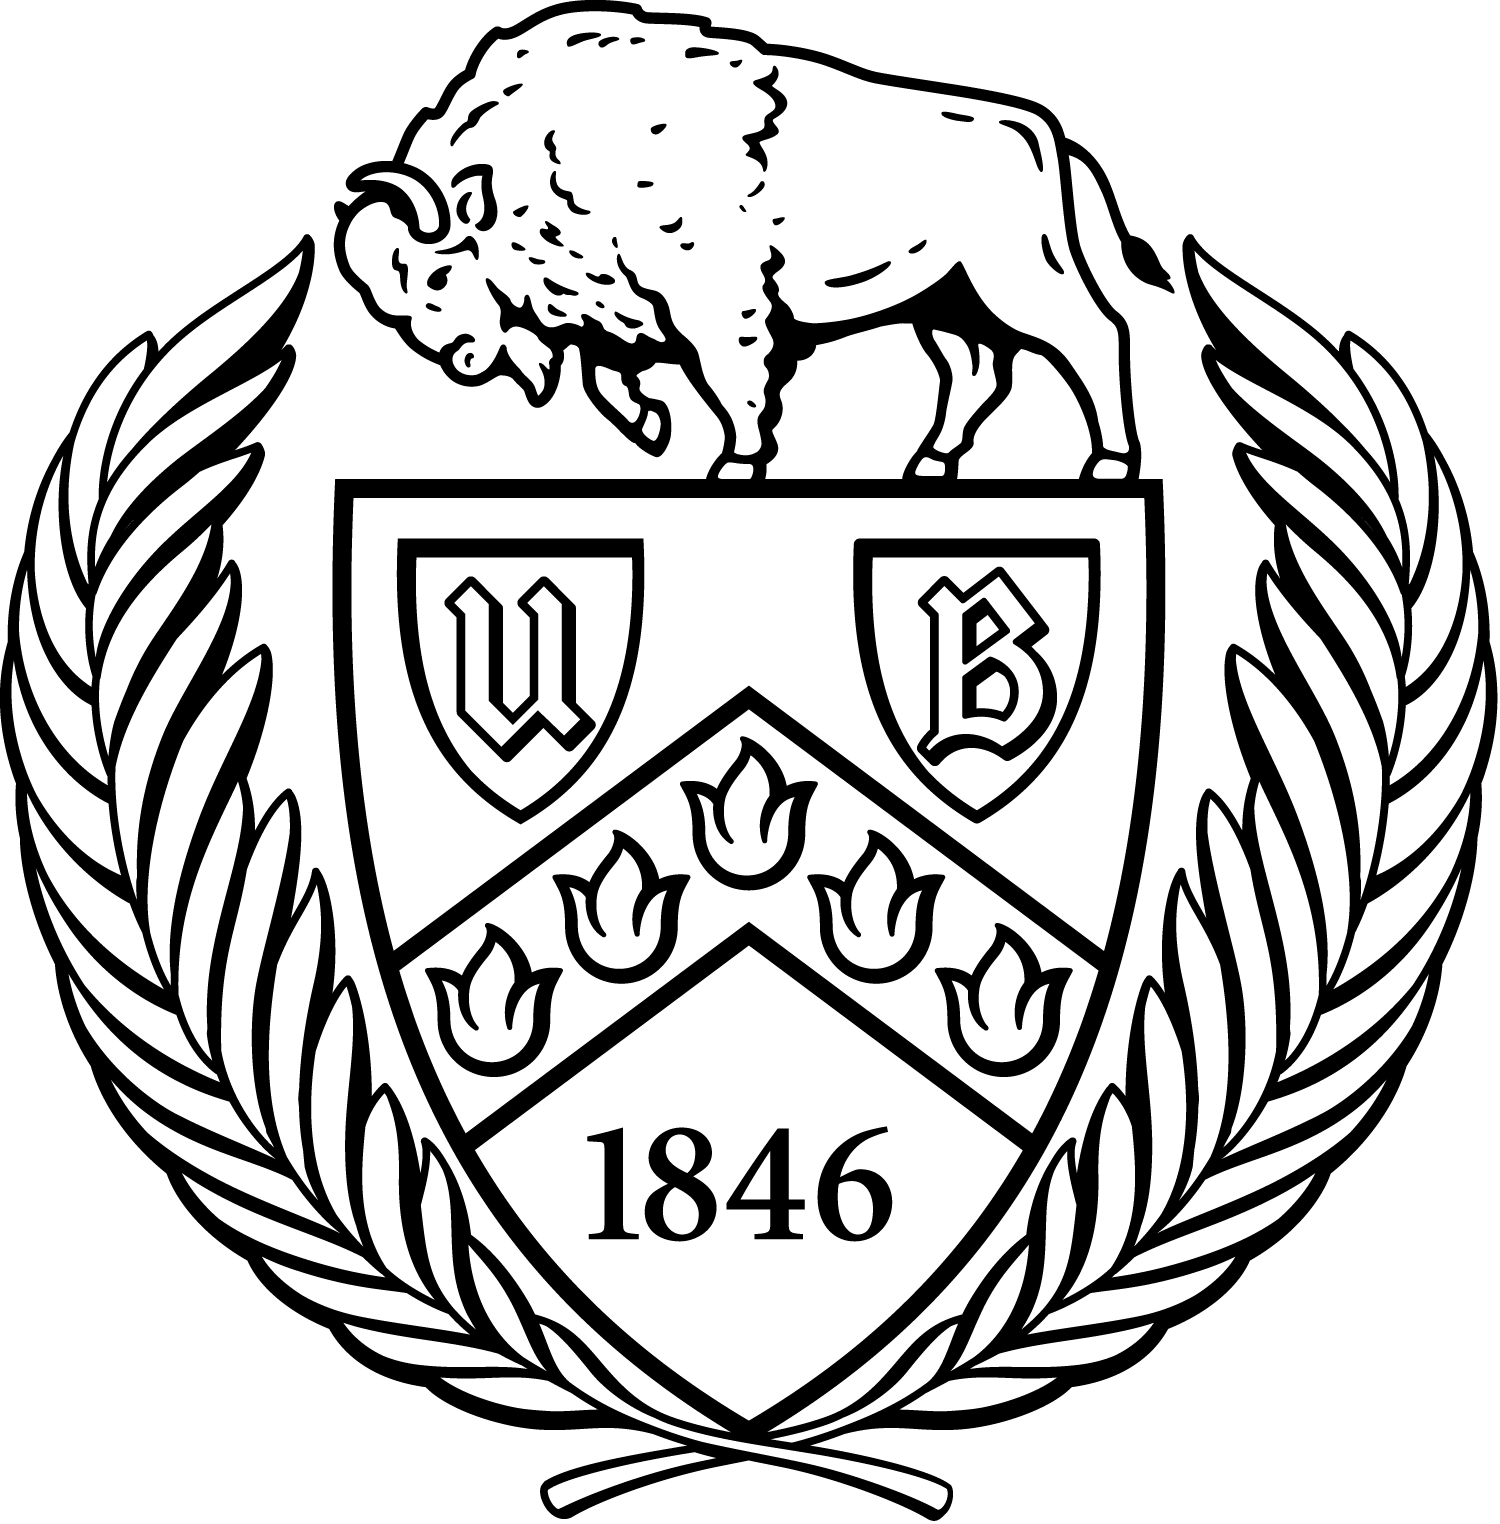
\includegraphics[
  width=6cm,
  height=6cm,
  keepaspectratio,
]{Crest_BW.png}\\[1cm] % Include a department/university logo - this will require the graphicx package
 
%----------------------------------------------------------------------------------------

\vfill % Fill the rest of the page with whitespace

\end{titlepage}

\title{\Large CSE 676: Deep Learning\\\Huge Assignment - 1}
\date{\today}
\author{Yash Narendra Saraf\\UB ID: 50290453\\\texttt{ysaraf@buffalo.edu}}
\maketitle
% //////////////////////////////////////////////////////////////////////////////////////////////////
% //////////////////////////////////////////////////////////////////////////////////////////////////
\section{Softmax [2 points]}

% //////////////////////////////////////////////////////////////////////////////////////////////////
\subsection{ [1 point] Prove that softmax is invariant to constant sifts in the input, i.e., for any
input vector x and a constant scalar c, the following holds: \\
$$ softmax(x) = softmax(x +c)  $$
 where $ softmax(x)_i \triangleq \dfrac{e^{x_i}}{\sum_{i_{'}}^{} e^{x_i^{'}}},$ and $ x +c $ means adding c to every dimension of x.}
 
 The definition of Softmax is - 
$$ softmax(x)_i \triangleq \dfrac{e^{x_i}}{\sum_{i_{'}}^{} e^{x_i^{'}}},$$

Now, we have to prove that even after constant shifts the output of the softmax won't change i.e.
$$ softmax(x) = softmax(x +c)  $$

So, replacing $x$ by $x+c$ in the original softmax equation, we have 
\begin{align*}
{softmax(x)_i &\triangleq \dfrac{e^{x_i}}{\sum_{i_{'}}^{} e^{x_i^{'}}}}\\
               &= \dfrac{e^{x_i + c}}{\sum_{i_{'}}^{} e^{x_i^{'}+c}}\\
               &= \dfrac{e^{c}*e^{x_i}}{e^{c} * \sum_{i_{'}}^{} e^{x_i^{'}}}\\
               &= \dfrac{e^{x_i}}{\sum_{i_{'}}^{} e^{x_i^{'}}}
\end{align*}

Hence Proved, softmax function is invariant to constant shifts. 

% //////////////////////////////////////////////////////////////////////////////////////////////////
\subsection{ [1 point] Let $z = W x + c$, where W and c are some matrix and vector, respectively.
Let \\
$$ J =  \sum_{i}^{}log  \, softmax(z_{i}) $$
 Calculate the derivatives of J w.r.t. W and c, respectively, i.e., calculate $ \frac{\partial J}{\partial W} $ and $ \frac{\partial J}{\partial c} $.}
 
 
For the calculation of $ \frac{\partial J}{\partial z} \ $, 

$$\frac{\partial J}{\partial z} =  -\frac{\partial}{\partial z} \ \sum_{i}^{}log  \, softmax(z_{i}) $$

Calculating the derivative by considering the derivative while doing calculations for Class i. 
This is necessary as when we use chain rule to calculate derivatives we will have different derivative for the class under considerations and all other classes. This is because of the derivative of the softmax function.  

$$\frac{\partial J}{\partial z} = -\frac{\partial}{\partial z}(log(softmax(z_i))) -\frac{\partial}{\partial z} \ \sum_{k\neq i}\, log(softmax(z_k))$$

$$\frac{\partial J}{\partial z} = -\Big(\frac{1}{(softmax(z_i))} \ \frac{\partial (softmax(z_i))}{\partial z}\Big) - \ \sum_{k\neq i}y_k \ \frac{1}{(softmax(z_k))} \frac{\partial (softmax(z_k))}{\partial z}$$


$$\frac{\partial J}{\partial z} = -(\ 1-(softmax(z_i))) + \ \sum_{k\neq i}\ (softmax(z_i))$$

$$\frac{\partial J}{\partial z} = -1 + (softmax(z_i)) + \ \sum_{k\neq i}(softmax(z_i))$$


$$\frac{\partial J(z)}{\partial z} = -1 + \ \Big(\sum_{k=1}^{N}1\Big) \ (softmax(z_i))$$


$$\frac{\partial J(z)}{\partial z} = -1 + \ N (softmax(z_i))$$ 

Now, we need to calculate the $ \frac{\partial J}{\partial W} $ and $ \frac{\partial J}{\partial c} $. This can be simply done by applying the chain rule as we know the values for $\frac{\partial J}{\partial z} $ and z. 

So, as  $z = W x + c$. 
We can write,  

$$\frac{\partial J}{\partial W}  = \frac{\partial J}{\partial z} \ \frac{\partial z}{\partial W}$$

$$\frac{\partial J}{\partial W}  = (-1 + \ N (softmax(z_i))) \ \frac{\partial z}{\partial W}$$

$$\frac{\partial J}{\partial W}  = (-1 + \ N (softmax(z_i))) \ x $$

and similarly for $ \frac{\partial J}{\partial c} $,


$$ \frac{\partial J}{\partial c}  = \frac{\partial J}{\partial z} \ \frac{\partial z}{\partial c}$$

$$\frac{\partial J}{\partial c}  = (-1 + \ N (softmax(z_i))) \ \frac{\partial z}{\partial c}$$

$$\frac{\partial J}{\partial c}  = (-1 + \ N (softmax(z_i))) \ $$


% //////////////////////////////////////////////////////////////////////////////////////////////////
% //////////////////////////////////////////////////////////////////////////////////////////////////
\section{Logistic Regression with Regularization [2 points]}
% //////////////////////////////////////////////////////////////////////////////////////////////////
\subsection{ [1 point] Let the data be $(x_i, y_i)_{i=1}^{N} $ where $ x_i \in R^{d} $ and $ y_i \in \{0,1\} $. Logistic regression is a binary classification model, with the probability of $y_i$ being 1 as:
$$ p(y_i;x_i,\theta) =  \sigma(\theta^Tx_i) \triangleq \dfrac{1}{1 + e^{-\theta^Tx_{i}}} $$
where $\theta$ is the model parameter. Assume we impose an L2 regularization term on the
parameter, defined as:
$$ R(\theta) = \dfrac{\lambda}{2}\theta^T\theta$$
with a positive constant $ \lambda$. Write out the final objective function for this logistic
regression with regularization model.
}

Let the given Hypothesis function be represented as - 

$$ h_\theta(x_i) = p(y_i = 1|x_i,\theta) =  \sigma(\theta^Tx_i) \triangleq \dfrac{1}{1 + e^{-\theta^Tx_{i}}} $$

and the Regularization term given is - 

$$ R(\theta) = \dfrac{\lambda}{2}\theta^T\theta$$

The above Hypothesis function gives the probability of predicting 1 for the given input. 

So, we can't use the Mean Square Error as the Loss function as it would not give convex function. So to solve this problem the loss function can be designed as following - 

$$ Cost(h_\theta(x_i), y_i) = -y_i\,log(h_\theta(x_i)) - (1-y_i)\,log(1-h_\theta(x_i))$$

Using the above cost function the Objective function can be designed as - 

$$J(\theta) = \frac{1}{N}\sum_{i=1}^{N}Cost(h_\theta(x_i), y_i) $$

The regularization term can be added to the equation, as the function of the regularizer is to make sure that the model does not overfit. It also makes sure that the value of weights remain as small as possible. There is a scaling factor involved with the regularization term to make sure that the regularizer does not hinder the model from learning just to minimize the weights. Let the parameter be $ \lambda $.

$$J(\theta) = \frac{1}{N}\sum_{i=1}^{N}Cost(h_\theta(x_i), y_i) \ + \  R(\theta)$$

The above function represents the Objective function for Logistic Regression Model. 

% //////////////////////////////////////////////////////////////////////////////////////////////////
\subsection{[1 point] If we use gradient descent to solve the model parameter. Derive the updating
rule for $\theta$ . Your answer should contain the derivation, not just the final answer}

Now, since we have obtained the Objective function, our goal is to use this function to find optimum weights for the model using Gradient Descent. The gradient descent algorithm tries to find the minima of the Objective function for optimization. Here, the minima can be easily found by derivating the cost function with respect to Weights i.e. $\theta$ and updating the weights. Derivating with respect to theta gives us the slope of the graph and we use the slope to travel to the minima of Objective function. 

So, we now have following equations - 


$$ h_\theta(x_i) = p(y_i = 1|x_i,\theta) =  \sigma(\theta^Tx_i) \triangleq \dfrac{1}{1 + e^{-\theta^Tx_{i}}} $$

$$ R(\theta) = \dfrac{\lambda}{2}\theta^T\theta$$

$$ Cost(h_\theta(x_i), y_i) = -y_i\,log(h_\theta(x_i)) - (1-y_i)\,log(1-h_\theta(x_i))$$

$$J(\theta) = \frac{1}{N}\sum_{i=1}^{N}Cost(h_\theta(x_i), y_i) \ + \  R(\theta)$$

To calculate gradient equation first let's just find derivative of Cost function. We can later substitute the same in the main equation for calculation of finding final gradient. 

$$ \frac{\partial Cost(h_\theta(x_i), y_i)}{\partial \theta_j} = -\Big(\frac{y_i}{h_\theta(x_i)} - \frac{1- y_i}{1 - h_\theta(x_i)}\Big) \ \frac{\partial \ h_\theta(x_i)}{\partial \ \theta_j} $$

Now, $h_\theta(x_i)$ is a sigmoid function and the derivative of sigmoid function is given by - 

$$ \frac{\partial Cost(h_\theta(x_i), y_i)}{\partial x} = h_\theta(x)(1-h_\theta(x))$$

So, using that updating our Gradient calculation, 

$$ \frac{\partial Cost(h_\theta(x_i), y_i)}{\partial \theta_j} = -\Big(\frac{y_i}{h_\theta(x_i)} - \frac{1- y_i}{1 - h_\theta(x_i)}\Big) \ h_\theta(x_i) \ (1-h_\theta(x_i)) \ \frac{\partial \ \theta^Tx_i}{\partial \ \theta_j} $$


$$ \frac{\partial Cost(h_\theta(x_i), y_i))}{\partial \theta_j} = -(y_i(1-h_\theta(x_i)) - (1-y_i)h_\theta(x_i)) \ x_{ij} $$

Here, $x_{ij}$ represents the $j^{th}$ weight when working with input $x_i$.    

$$ \frac{\partial Cost(h_\theta(x_i), y_i)}{\partial \theta_j} = -(y_i - h_\theta(x_i)) \ x_{ij} $$

Now, calculating the complete gradient equation using the above partial derivative. 

So, 

$$ \frac{\partial J(\theta)}{\partial \theta_j} = \frac{\partial}{\partial \theta_j} \Big(\frac{1}{N}\sum_{i=1}^{N}Cost(h_\theta(x_i), y_i) \ + \  R(\theta)\Big)$$


$$ \frac{\partial J(\theta)}{\partial \theta_j} =\frac{1}{N}\sum_{i=1}^{N} \frac{\partial}{\partial \theta_j} \ Cost(h_\theta(x_i), y_i) \ + \ \frac{\partial}{\partial \theta_j} R(\theta)$$


$$ \frac{\partial J(\theta)}{\partial \theta_j} =-\frac{1}{N}\sum_{i=1}^{N} (y_i - h_\theta(x_i)) \ x_{ij} \ + \ \frac{\partial}{\partial \theta_j} R(\theta)$$


$$ \frac{\partial J(\theta)}{\partial \theta_j} =-\frac{1}{N}\sum_{i=1}^{N} (y_i - h_\theta(x_i)) \ x_{ij} \ + \  \frac{\partial}{\partial \theta_j} R(\theta)$$

Now, calculating the derivative of Regularization term - 

$$ \frac{\partial}{\partial \theta_j} R(\theta) = \frac{\partial}{\partial \theta_j} \  \dfrac{\lambda}{2}\theta^T\theta $$ 

$$ \frac{\partial}{\partial \theta_j} R(\theta) = \dfrac{\lambda}{2} \ \frac{\partial}{\partial \theta_j} (\theta^T\theta) $$

$$ \frac{\partial}{\partial \theta_j} R(\theta) = \dfrac{\lambda}{2} \ (2 \ \theta_j) $$

$$ \frac{\partial}{\partial \theta_j} R(\theta) = \lambda \ \theta_j$$

Substituting, the same in the gradient equation. 

$$ \frac{\partial J(\theta)}{\partial \theta_j} =-\frac{1}{N}\sum_{i=1}^{N} (y_i - h_\theta(x_i)) \ x_{ij} \ + \  \lambda \ \theta_j$$

So, weight updation equation will look like, 

$$ \theta_j = \theta_j - \alpha \ \frac{\partial J(\theta)}{\partial \theta_j} $$

$$ \theta_j = \theta_j - \alpha \ (-\frac{1}{N}\sum_{i=1}^{N} (y_i - h_\theta(x_i)) \ x_{ij} \ + \  \lambda \ \theta_j) $$

$$ \theta_j = \theta_j - \alpha \ (\frac{1}{N}\sum_{i=1}^{N} (h_\theta(x_i)-y_i) \ x_{ij} \ + \  \lambda \ \theta_j) $$

The constants can be combined and the final equation looks like - 

$$ \theta_j = \theta_j\Big(1-\frac{\lambda}{N}\Big) - \alpha \ (\sum_{i=1}^{N} (h_\theta(x_i)-y_i) \ x_{ij}) $$

In, the above equation the $\lambda$ represents the regularization constant and $\alpha$ represents the learning rate. 

% //////////////////////////////////////////////////////////////////////////////////////////////////
% //////////////////////////////////////////////////////////////////////////////////////////////////
\section{Derivative of the Softmax Function [3 points]}

% //////////////////////////////////////////////////////////////////////////////////////////////////
\subsection{ [1 point] Define the loss function as 
$$ J(z) = -\sum_{k=1}^{K}y_k \, log \widetilde{y}_k $$ 
where  $\widetilde{y}_k = \dfrac{e^{z_k}}{\sum_{k^{'}}^{} e^{z_{k^{'}}}}$ , and $(y_1,.., y_K)$ is a known probability vector. Derive the  $ \frac{\partial J(z)}{\partial z} $.
Note  $z = (z_1,.., z_K)$ is a vector so  $ \frac{\partial J(z)}{\partial z} $ is in the form of a vector. Your answer should contain the derivation, not just the final answer.}

For the calculation of $ \frac{\partial J(z)}{\partial z} \ $, 

$$\frac{\partial J(z)}{\partial z} =  -\frac{\partial}{\partial z} \ \sum_{k=1}^{K}y_k \, log \widetilde{y}_k$$

Calculating the derivative by considering the derivative while doing calculations for Class i. 
This is necessary as when we use chain rule to calculate derivatives we will have different derivative for the class under considerations and all other classes. This is because of the derivative of the softmax function.  

$$\frac{\partial J(z)}{\partial z} = -\frac{\partial}{\partial z}(y_i \ log(\widetilde{y}_i)) -\frac{\partial}{\partial z} \ \sum_{k\neq i}y_k \, log \widetilde{y}_k$$

$$\frac{\partial J(z)}{\partial z} = -\Big(y_i \ \frac{1}{\widetilde{y}_i} \ \frac{\partial y_i}{\partial z}\Big) - \ \sum_{k\neq i}y_k \ \frac{1}{\widetilde{y}_k} \frac{\partial \widetilde{y}_k}{\partial z}$$



$$\frac{\partial J(z)}{\partial z} = -(y_i \ (1-\widetilde{y}_i)) + \ \sum_{k\neq i}y_k \ \widetilde{y}_i$$

$$\frac{\partial J(z)}{\partial z} = -y_i + y_i \ \widetilde{y}_i + \ \sum_{k\neq i}y_k \ \widetilde{y}_i$$


$$\frac{\partial J(z)}{\partial z} = -y_i + \ \Big(\sum_{k=1}^{N}y_k\Big) \ \widetilde{y}_i$$


$$\frac{\partial J(z)}{\partial z} = -y_i + \ \widetilde{y}_i$$

% //////////////////////////////////////////////////////////////////////////////////////////////////
\subsection{ [1 point] Assume the above softmax is the output layer of an FNN. Briefly explain
how the derivative is used in the back propagation algorithm.}

In the above answer, the J(z) function given is the Cross Entropy Loss function. So we found the derivative of the Cross Entropy with respect to the output of the final layer i.e. $ \frac{\partial J(z)}{\partial z} $ as $ z = W^T \ h + b$. So, now we know gradient for the last layer. 

Now, to when we update the value of each weights i.e. $W_{ij}$, where W is the node from Node i to Node j, we need the value of $ \frac{\partial J(z)}{\partial W_{ij}} $, so to calculate which there is a need to propagate the error calculated at the last layer, and use chain rule in Calculus to propagate the error backwards.. 

The $ \frac{\partial J(z)}{\partial W_{ij}} $ is calculated for each weight and all weights are updated for that particular iteration. 

The property of the loss function for softmax regression is that it only penalizes the output from the correct class. But when we calculate the gradient equation it can be seen that all the the incorrect classes also get affected based on how incorrect those classes are. 

% //////////////////////////////////////////////////////////////////////////////////////////////////
\subsection{ [1 points] Let $z = W^T h + b$, where W is a matrix, b and h are vectors. Use the
chain rule to calculate the gradient of W and b, i.e.,
$ \frac{\partial J}{\partial W} $ and $ \frac{\partial J}{\partial b} $, respectively}

In the first part we calculated the following, 

$$\frac{\partial J(z)}{\partial z} = -y_i + \ \widetilde{y}_i$$.

Now, if we need to calculate $ \frac{\partial J}{\partial W} $ and $ \frac{\partial J}{\partial b} $, we can simply use $z = W^T h + b$ and update based on this. 

So, 

$$ \frac{\partial J(z)}{\partial W}  =  \frac{\partial J(z)}{\partial z} \ \frac{\partial z}{\partial W} $$

$$ \frac{\partial J(z)}{\partial W}  =   (-y_i + \ \widetilde{y}_i)\ \frac{\partial z}{\partial W} $$

$$ \frac{\partial J(z)}{\partial W}  =   (-y_i + \ \widetilde{y}_i)\ \frac{\partial (W^T h + b)}{\partial W} $$


$$ \frac{\partial J(z)}{\partial W}  =   (-y_i + \ \widetilde{y}_i)\ \frac{\partial (W^T h + b)}{\partial W} $$


$$ \frac{\partial J(z)}{\partial W}  =   (-y_i + \ \widetilde{y}_i) \ h $$

and similarly for $ \frac{\partial J}{\partial b} $, 

$$ \frac{\partial J(z)}{\partial b}  =   (-y_i + \ \widetilde{y}_i)\ \frac{\partial (W^T h + b)}{\partial b} $$

$$ \frac{\partial J(z)}{\partial b}  =   (-y_i + \ \widetilde{y}_i) $$

% //////////////////////////////////////////////////////////////////////////////////////////////////
% //////////////////////////////////////////////////////////////////////////////////////////////////
\section{MNIST with FNN [3 points]}

% //////////////////////////////////////////////////////////////////////////////////////////////////
\subsection{[3 points] Design an FNN for MNIST classification. Implement the model and plot
two curves in one figure: i) training loss vs. training iterations; ii) test loss vs. training
iterations.\\
– You can use code from websites. However, you must reference (cite) the code in
your answer.\\
– Submission includes the plot of the two curves and the runnable code (with a
ReadMe file containing instructions on how to run the code).}

For this question code can be found in the submitted folder directory. 
The ReadMe has also been added for reference. \\
The name of the file is \textbf{Q4\_MNIST\_FNN.ipynb}\\
The code is written inside jupyter notebook. Also for reference the tensorflow tutorials slides were used along with this \href{https://github.com/aymericdamien/TensorFlow-Examples/blob/master/examples/3_NeuralNetworks/multilayer_perceptron.py}{GitHub Repository}. 




The result graphs for the code can be found below - \\
\begin{figure}[h]
\centering
\begin{minipage}{.5\textwidth}
  \centering
  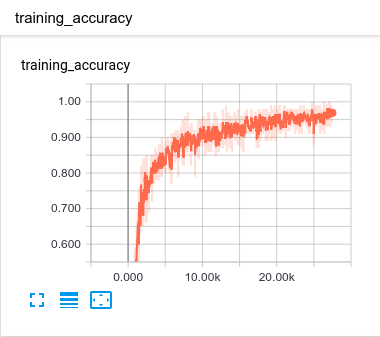
\includegraphics[width=.99\linewidth]{1.png}
  \captionof{}{Training Accuracy Graph}
\end{minipage}%
\begin{minipage}{.5\textwidth}
  \centering
  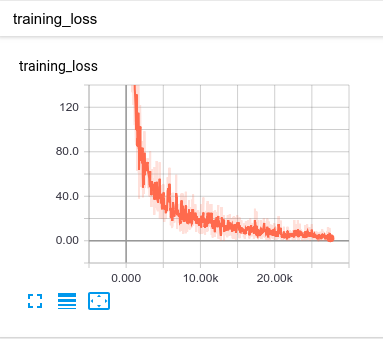
\includegraphics[width=.99\linewidth]{2.png}
  \captionof{}{Training Cost Graph}
\end{minipage}
\end{figure}

\begin{figure}[h]
\centering
\begin{minipage}{.5\textwidth}
  \centering
  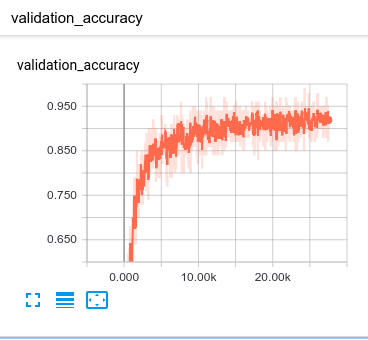
\includegraphics[width=.99\linewidth]{3.png}
  \captionof{}{Validation Accuracy Graph}
\end{minipage}%
\begin{minipage}{.5\textwidth}
  \centering
  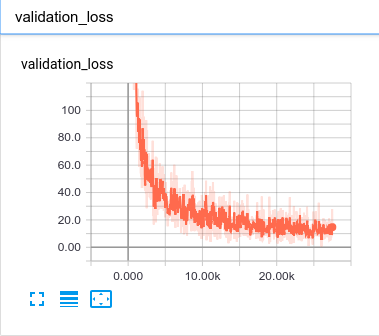
\includegraphics[width=.99\linewidth]{4.png}
  \captionof{}{Validation Cost Graph}
\end{minipage}
\end{figure}
    
\end{document} to your LaTeX file where you want your
% title page.
%
%%%%%%%%%%%%%%%%%%%%%%%%%%%%%%%%%%%%%%%%%
%\title{Title page with logo}
%----------------------------------------------------------------------------------------
%	PACKAGES AND OTHER DOCUMENT CONFIGURATIONS
%----------------------------------------------------------------------------------------

\documentclass[12]{article}
\usepackage[letterpaper, margin=0.5in, top=0.5in]{geometry}
\usepackage{enumitem}
\usepackage{mathtools}
\usepackage{amssymb}
% \usepackage{amsmath}
\usepackage{listings}
\usepackage{color}
\usepackage{cancel}
\usepackage{paracol}
\usepackage{dcolumn}
\usepackage[english]{babel}
\usepackage[utf8x]{inputenc}
\usepackage{amsmath}
\usepackage{graphicx}
\usepackage[colorinlistoftodos]{todonotes}
\usepackage{hyperref}

\renewcommand{\thesection}{Q\arabic{section}}
\renewcommand{\thesubsection}{(\arabic{subsection})}
\newcommand{\equno}[1]{\ensuremath{\stepcounter{equation}\tag{\theequation}\label{#1}}}
\newcommand{\bref}[1]{\textbf{\texttt{#1}}}

\definecolor{codeGray}{rgb}{0.8,0.8,0.8}
\lstdefinestyle{codeBlock}{
	backgroundcolor=\color{codeGray},
	frame=single,
	tabsize=2,
	captionpos=b
}
\hypersetup{
    colorlinks=true,
    linkcolor=blue,
    filecolor=magenta,      
    urlcolor=cyan,
}
\lstset{style=codeBlock}

\begin{document}

\begin{titlepage}

\newcommand{\HRule}{\rule{\linewidth}{0.5mm}} % Defines a new command for the horizontal lines, change thickness here

\center % Center everything on the page
 
%----------------------------------------------------------------------------------------
%	HEADING SECTIONS
%----------------------------------------------------------------------------------------
\vspace*{150px}
\textsc{\LARGE University at Buffalo, \\The State University of New York}\\[1.5cm] % Name of your university/college
\textsc{\large CSE 676}\\[0.5cm] % Major heading such as course name
\textsc{\large Deep Learning}\\[0.5cm] % Minor heading such as course title

%----------------------------------------------------------------------------------------
%	TITLE SECTION
%----------------------------------------------------------------------------------------

\HRule \\[0.4cm]
{ \LARGE \bfseries Assignment - 1}\\[0.4cm] % Title of your document
\HRule \\[1.5cm]
 
%----------------------------------------------------------------------------------------
%	AUTHOR SECTION
%----------------------------------------------------------------------------------------

\begin{center}
% \emph{Author:}\\
\Large Yash Narendra Saraf (50290453)\\
\end{center}


% If you don't want a supervisor, uncomment the two lines below and remove the section above
%\Large \emph{Author:}\\
%John \textsc{Smith}\\[3cm] % Your name

%----------------------------------------------------------------------------------------
%	DATE SECTION
%----------------------------------------------------------------------------------------
% Date, change the \today to a set date if you want to be precise

%----------------------------------------------------------------------------------------
%	LOGO SECTION
%----------------------------------------------------------------------------------------

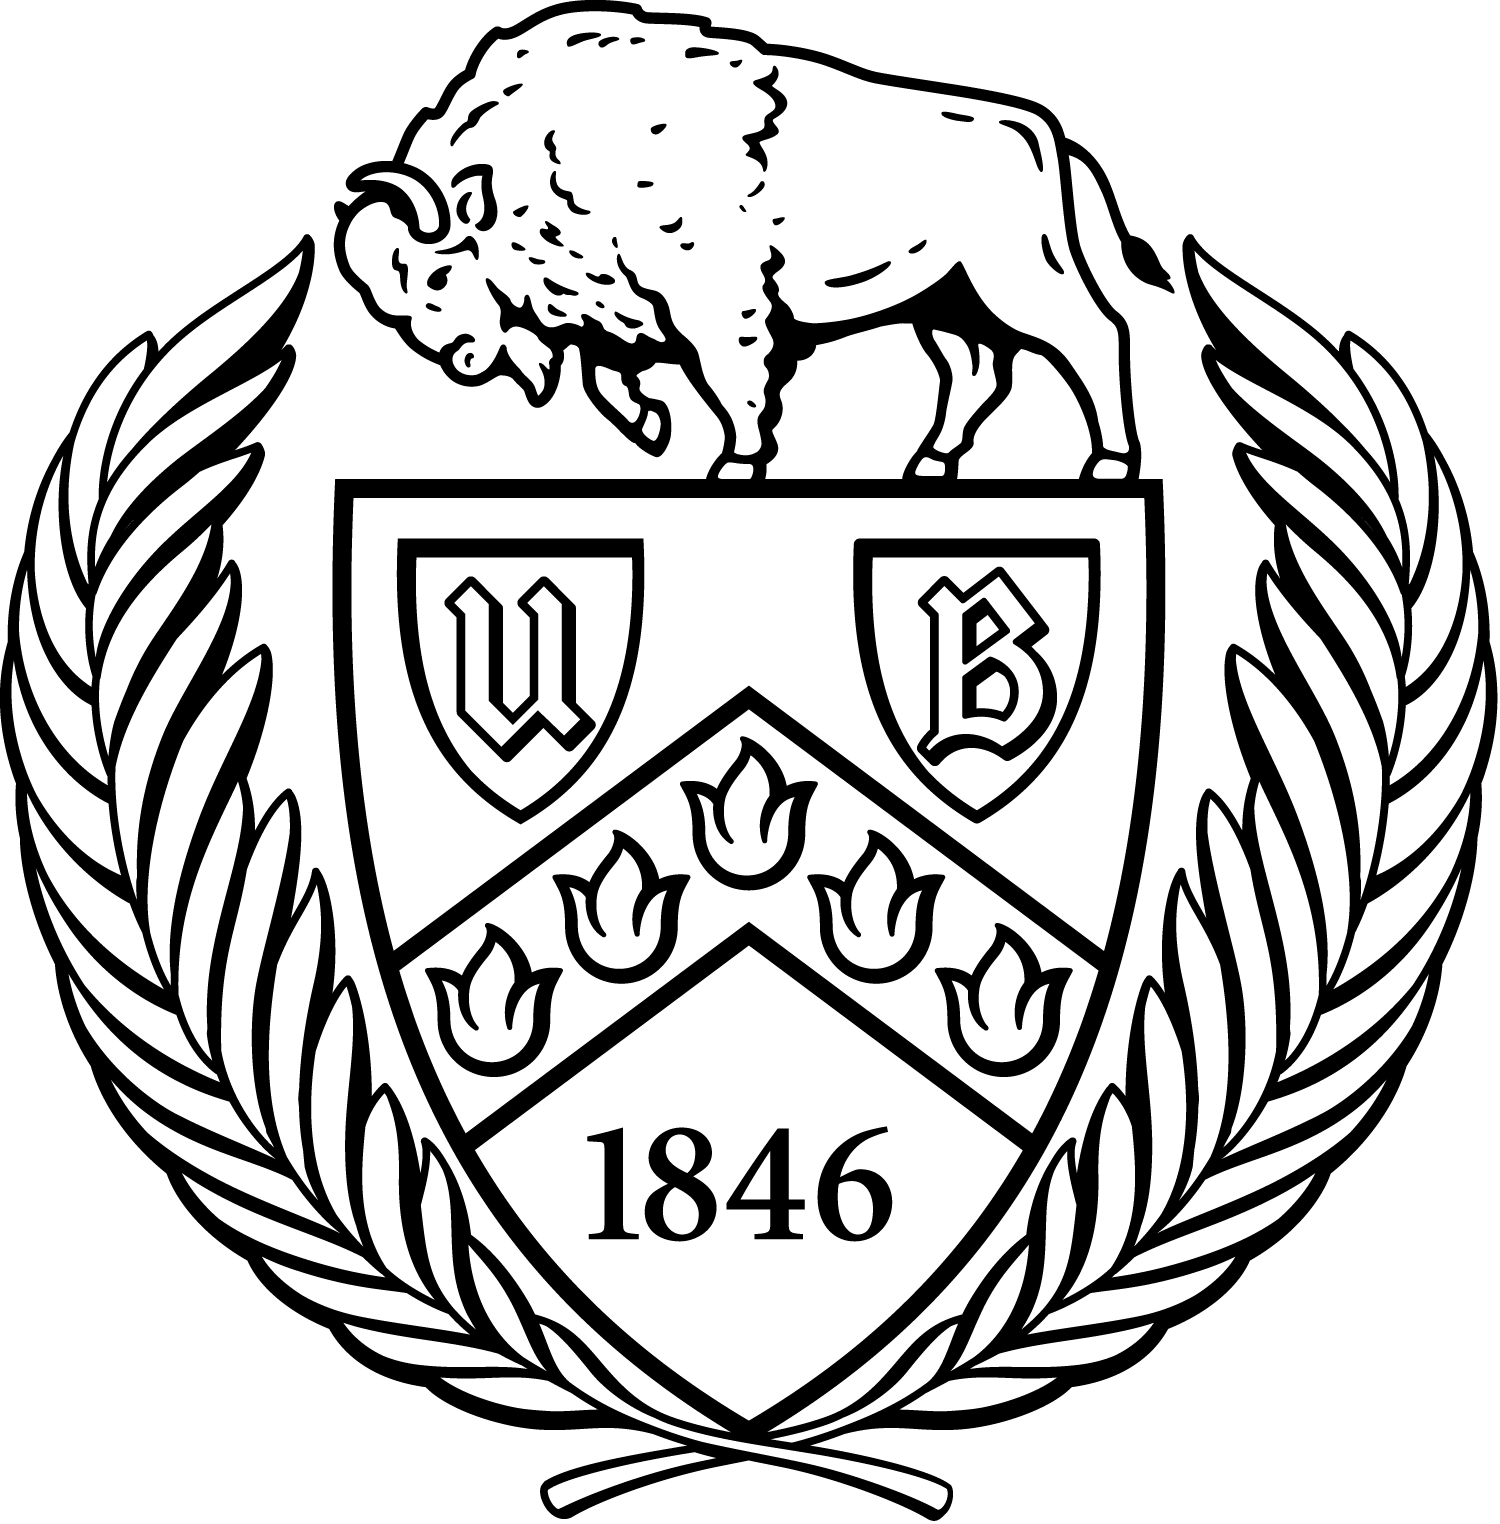
\includegraphics[
  width=6cm,
  height=6cm,
  keepaspectratio,
]{Crest_BW.png}\\[1cm] % Include a department/university logo - this will require the graphicx package
 
%----------------------------------------------------------------------------------------

\vfill % Fill the rest of the page with whitespace

\end{titlepage}

\title{\Large CSE 676: Deep Learning\\\Huge Assignment - 1}
\date{\today}
\author{Yash Narendra Saraf\\UB ID: 50290453\\\texttt{ysaraf@buffalo.edu}}
\maketitle
% //////////////////////////////////////////////////////////////////////////////////////////////////
% //////////////////////////////////////////////////////////////////////////////////////////////////
\section{Softmax [2 points]}

% //////////////////////////////////////////////////////////////////////////////////////////////////
\subsection{ [1 point] Prove that softmax is invariant to constant sifts in the input, i.e., for any
input vector x and a constant scalar c, the following holds: \\
$$ softmax(x) = softmax(x +c)  $$
 where $ softmax(x)_i \triangleq \dfrac{e^{x_i}}{\sum_{i_{'}}^{} e^{x_i^{'}}},$ and $ x +c $ means adding c to every dimension of x.}
 
 The definition of Softmax is - 
$$ softmax(x)_i \triangleq \dfrac{e^{x_i}}{\sum_{i_{'}}^{} e^{x_i^{'}}},$$

Now, we have to prove that even after constant shifts the output of the softmax won't change i.e.
$$ softmax(x) = softmax(x +c)  $$

So, replacing $x$ by $x+c$ in the original softmax equation, we have 
\begin{align*}
{softmax(x)_i &\triangleq \dfrac{e^{x_i}}{\sum_{i_{'}}^{} e^{x_i^{'}}}}\\
               &= \dfrac{e^{x_i + c}}{\sum_{i_{'}}^{} e^{x_i^{'}+c}}\\
               &= \dfrac{e^{c}*e^{x_i}}{e^{c} * \sum_{i_{'}}^{} e^{x_i^{'}}}\\
               &= \dfrac{e^{x_i}}{\sum_{i_{'}}^{} e^{x_i^{'}}}
\end{align*}

Hence Proved, softmax function is invariant to constant shifts. 

% //////////////////////////////////////////////////////////////////////////////////////////////////
\subsection{ [1 point] Let $z = W x + c$, where W and c are some matrix and vector, respectively.
Let \\
$$ J =  \sum_{i}^{}log  \, softmax(z_{i}) $$
 Calculate the derivatives of J w.r.t. W and c, respectively, i.e., calculate $ \frac{\partial J}{\partial W} $ and $ \frac{\partial J}{\partial c} $.}
 
 
For the calculation of $ \frac{\partial J}{\partial z} \ $, 

$$\frac{\partial J}{\partial z} =  -\frac{\partial}{\partial z} \ \sum_{i}^{}log  \, softmax(z_{i}) $$

Calculating the derivative by considering the derivative while doing calculations for Class i. 
This is necessary as when we use chain rule to calculate derivatives we will have different derivative for the class under considerations and all other classes. This is because of the derivative of the softmax function.  

$$\frac{\partial J}{\partial z} = -\frac{\partial}{\partial z}(log(softmax(z_i))) -\frac{\partial}{\partial z} \ \sum_{k\neq i}\, log(softmax(z_k))$$

$$\frac{\partial J}{\partial z} = -\Big(\frac{1}{(softmax(z_i))} \ \frac{\partial (softmax(z_i))}{\partial z}\Big) - \ \sum_{k\neq i}y_k \ \frac{1}{(softmax(z_k))} \frac{\partial (softmax(z_k))}{\partial z}$$


$$\frac{\partial J}{\partial z} = -(\ 1-(softmax(z_i))) + \ \sum_{k\neq i}\ (softmax(z_i))$$

$$\frac{\partial J}{\partial z} = -1 + (softmax(z_i)) + \ \sum_{k\neq i}(softmax(z_i))$$


$$\frac{\partial J(z)}{\partial z} = -1 + \ \Big(\sum_{k=1}^{N}1\Big) \ (softmax(z_i))$$


$$\frac{\partial J(z)}{\partial z} = -1 + \ N (softmax(z_i))$$ 

Now, we need to calculate the $ \frac{\partial J}{\partial W} $ and $ \frac{\partial J}{\partial c} $. This can be simply done by applying the chain rule as we know the values for $\frac{\partial J}{\partial z} $ and z. 

So, as  $z = W x + c$. 
We can write,  

$$\frac{\partial J}{\partial W}  = \frac{\partial J}{\partial z} \ \frac{\partial z}{\partial W}$$

$$\frac{\partial J}{\partial W}  = (-1 + \ N (softmax(z_i))) \ \frac{\partial z}{\partial W}$$

$$\frac{\partial J}{\partial W}  = (-1 + \ N (softmax(z_i))) \ x $$

and similarly for $ \frac{\partial J}{\partial c} $,


$$ \frac{\partial J}{\partial c}  = \frac{\partial J}{\partial z} \ \frac{\partial z}{\partial c}$$

$$\frac{\partial J}{\partial c}  = (-1 + \ N (softmax(z_i))) \ \frac{\partial z}{\partial c}$$

$$\frac{\partial J}{\partial c}  = (-1 + \ N (softmax(z_i))) \ $$


% //////////////////////////////////////////////////////////////////////////////////////////////////
% //////////////////////////////////////////////////////////////////////////////////////////////////
\section{Logistic Regression with Regularization [2 points]}
% //////////////////////////////////////////////////////////////////////////////////////////////////
\subsection{ [1 point] Let the data be $(x_i, y_i)_{i=1}^{N} $ where $ x_i \in R^{d} $ and $ y_i \in \{0,1\} $. Logistic regression is a binary classification model, with the probability of $y_i$ being 1 as:
$$ p(y_i;x_i,\theta) =  \sigma(\theta^Tx_i) \triangleq \dfrac{1}{1 + e^{-\theta^Tx_{i}}} $$
where $\theta$ is the model parameter. Assume we impose an L2 regularization term on the
parameter, defined as:
$$ R(\theta) = \dfrac{\lambda}{2}\theta^T\theta$$
with a positive constant $ \lambda$. Write out the final objective function for this logistic
regression with regularization model.
}

Let the given Hypothesis function be represented as - 

$$ h_\theta(x_i) = p(y_i = 1|x_i,\theta) =  \sigma(\theta^Tx_i) \triangleq \dfrac{1}{1 + e^{-\theta^Tx_{i}}} $$

and the Regularization term given is - 

$$ R(\theta) = \dfrac{\lambda}{2}\theta^T\theta$$

The above Hypothesis function gives the probability of predicting 1 for the given input. 

So, we can't use the Mean Square Error as the Loss function as it would not give convex function. So to solve this problem the loss function can be designed as following - 

$$ Cost(h_\theta(x_i), y_i) = -y_i\,log(h_\theta(x_i)) - (1-y_i)\,log(1-h_\theta(x_i))$$

Using the above cost function the Objective function can be designed as - 

$$J(\theta) = \frac{1}{N}\sum_{i=1}^{N}Cost(h_\theta(x_i), y_i) $$

The regularization term can be added to the equation, as the function of the regularizer is to make sure that the model does not overfit. It also makes sure that the value of weights remain as small as possible. There is a scaling factor involved with the regularization term to make sure that the regularizer does not hinder the model from learning just to minimize the weights. Let the parameter be $ \lambda $.

$$J(\theta) = \frac{1}{N}\sum_{i=1}^{N}Cost(h_\theta(x_i), y_i) \ + \  R(\theta)$$

The above function represents the Objective function for Logistic Regression Model. 

% //////////////////////////////////////////////////////////////////////////////////////////////////
\subsection{[1 point] If we use gradient descent to solve the model parameter. Derive the updating
rule for $\theta$ . Your answer should contain the derivation, not just the final answer}

Now, since we have obtained the Objective function, our goal is to use this function to find optimum weights for the model using Gradient Descent. The gradient descent algorithm tries to find the minima of the Objective function for optimization. Here, the minima can be easily found by derivating the cost function with respect to Weights i.e. $\theta$ and updating the weights. Derivating with respect to theta gives us the slope of the graph and we use the slope to travel to the minima of Objective function. 

So, we now have following equations - 


$$ h_\theta(x_i) = p(y_i = 1|x_i,\theta) =  \sigma(\theta^Tx_i) \triangleq \dfrac{1}{1 + e^{-\theta^Tx_{i}}} $$

$$ R(\theta) = \dfrac{\lambda}{2}\theta^T\theta$$

$$ Cost(h_\theta(x_i), y_i) = -y_i\,log(h_\theta(x_i)) - (1-y_i)\,log(1-h_\theta(x_i))$$

$$J(\theta) = \frac{1}{N}\sum_{i=1}^{N}Cost(h_\theta(x_i), y_i) \ + \  R(\theta)$$

To calculate gradient equation first let's just find derivative of Cost function. We can later substitute the same in the main equation for calculation of finding final gradient. 

$$ \frac{\partial Cost(h_\theta(x_i), y_i)}{\partial \theta_j} = -\Big(\frac{y_i}{h_\theta(x_i)} - \frac{1- y_i}{1 - h_\theta(x_i)}\Big) \ \frac{\partial \ h_\theta(x_i)}{\partial \ \theta_j} $$

Now, $h_\theta(x_i)$ is a sigmoid function and the derivative of sigmoid function is given by - 

$$ \frac{\partial Cost(h_\theta(x_i), y_i)}{\partial x} = h_\theta(x)(1-h_\theta(x))$$

So, using that updating our Gradient calculation, 

$$ \frac{\partial Cost(h_\theta(x_i), y_i)}{\partial \theta_j} = -\Big(\frac{y_i}{h_\theta(x_i)} - \frac{1- y_i}{1 - h_\theta(x_i)}\Big) \ h_\theta(x_i) \ (1-h_\theta(x_i)) \ \frac{\partial \ \theta^Tx_i}{\partial \ \theta_j} $$


$$ \frac{\partial Cost(h_\theta(x_i), y_i))}{\partial \theta_j} = -(y_i(1-h_\theta(x_i)) - (1-y_i)h_\theta(x_i)) \ x_{ij} $$

Here, $x_{ij}$ represents the $j^{th}$ weight when working with input $x_i$.    

$$ \frac{\partial Cost(h_\theta(x_i), y_i)}{\partial \theta_j} = -(y_i - h_\theta(x_i)) \ x_{ij} $$

Now, calculating the complete gradient equation using the above partial derivative. 

So, 

$$ \frac{\partial J(\theta)}{\partial \theta_j} = \frac{\partial}{\partial \theta_j} \Big(\frac{1}{N}\sum_{i=1}^{N}Cost(h_\theta(x_i), y_i) \ + \  R(\theta)\Big)$$


$$ \frac{\partial J(\theta)}{\partial \theta_j} =\frac{1}{N}\sum_{i=1}^{N} \frac{\partial}{\partial \theta_j} \ Cost(h_\theta(x_i), y_i) \ + \ \frac{\partial}{\partial \theta_j} R(\theta)$$


$$ \frac{\partial J(\theta)}{\partial \theta_j} =-\frac{1}{N}\sum_{i=1}^{N} (y_i - h_\theta(x_i)) \ x_{ij} \ + \ \frac{\partial}{\partial \theta_j} R(\theta)$$


$$ \frac{\partial J(\theta)}{\partial \theta_j} =-\frac{1}{N}\sum_{i=1}^{N} (y_i - h_\theta(x_i)) \ x_{ij} \ + \  \frac{\partial}{\partial \theta_j} R(\theta)$$

Now, calculating the derivative of Regularization term - 

$$ \frac{\partial}{\partial \theta_j} R(\theta) = \frac{\partial}{\partial \theta_j} \  \dfrac{\lambda}{2}\theta^T\theta $$ 

$$ \frac{\partial}{\partial \theta_j} R(\theta) = \dfrac{\lambda}{2} \ \frac{\partial}{\partial \theta_j} (\theta^T\theta) $$

$$ \frac{\partial}{\partial \theta_j} R(\theta) = \dfrac{\lambda}{2} \ (2 \ \theta_j) $$

$$ \frac{\partial}{\partial \theta_j} R(\theta) = \lambda \ \theta_j$$

Substituting, the same in the gradient equation. 

$$ \frac{\partial J(\theta)}{\partial \theta_j} =-\frac{1}{N}\sum_{i=1}^{N} (y_i - h_\theta(x_i)) \ x_{ij} \ + \  \lambda \ \theta_j$$

So, weight updation equation will look like, 

$$ \theta_j = \theta_j - \alpha \ \frac{\partial J(\theta)}{\partial \theta_j} $$

$$ \theta_j = \theta_j - \alpha \ (-\frac{1}{N}\sum_{i=1}^{N} (y_i - h_\theta(x_i)) \ x_{ij} \ + \  \lambda \ \theta_j) $$

$$ \theta_j = \theta_j - \alpha \ (\frac{1}{N}\sum_{i=1}^{N} (h_\theta(x_i)-y_i) \ x_{ij} \ + \  \lambda \ \theta_j) $$

The constants can be combined and the final equation looks like - 

$$ \theta_j = \theta_j\Big(1-\frac{\lambda}{N}\Big) - \alpha \ (\sum_{i=1}^{N} (h_\theta(x_i)-y_i) \ x_{ij}) $$

In, the above equation the $\lambda$ represents the regularization constant and $\alpha$ represents the learning rate. 

% //////////////////////////////////////////////////////////////////////////////////////////////////
% //////////////////////////////////////////////////////////////////////////////////////////////////
\section{Derivative of the Softmax Function [3 points]}

% //////////////////////////////////////////////////////////////////////////////////////////////////
\subsection{ [1 point] Define the loss function as 
$$ J(z) = -\sum_{k=1}^{K}y_k \, log \widetilde{y}_k $$ 
where  $\widetilde{y}_k = \dfrac{e^{z_k}}{\sum_{k^{'}}^{} e^{z_{k^{'}}}}$ , and $(y_1,.., y_K)$ is a known probability vector. Derive the  $ \frac{\partial J(z)}{\partial z} $.
Note  $z = (z_1,.., z_K)$ is a vector so  $ \frac{\partial J(z)}{\partial z} $ is in the form of a vector. Your answer should contain the derivation, not just the final answer.}

For the calculation of $ \frac{\partial J(z)}{\partial z} \ $, 

$$\frac{\partial J(z)}{\partial z} =  -\frac{\partial}{\partial z} \ \sum_{k=1}^{K}y_k \, log \widetilde{y}_k$$

Calculating the derivative by considering the derivative while doing calculations for Class i. 
This is necessary as when we use chain rule to calculate derivatives we will have different derivative for the class under considerations and all other classes. This is because of the derivative of the softmax function.  

$$\frac{\partial J(z)}{\partial z} = -\frac{\partial}{\partial z}(y_i \ log(\widetilde{y}_i)) -\frac{\partial}{\partial z} \ \sum_{k\neq i}y_k \, log \widetilde{y}_k$$

$$\frac{\partial J(z)}{\partial z} = -\Big(y_i \ \frac{1}{\widetilde{y}_i} \ \frac{\partial y_i}{\partial z}\Big) - \ \sum_{k\neq i}y_k \ \frac{1}{\widetilde{y}_k} \frac{\partial \widetilde{y}_k}{\partial z}$$



$$\frac{\partial J(z)}{\partial z} = -(y_i \ (1-\widetilde{y}_i)) + \ \sum_{k\neq i}y_k \ \widetilde{y}_i$$

$$\frac{\partial J(z)}{\partial z} = -y_i + y_i \ \widetilde{y}_i + \ \sum_{k\neq i}y_k \ \widetilde{y}_i$$


$$\frac{\partial J(z)}{\partial z} = -y_i + \ \Big(\sum_{k=1}^{N}y_k\Big) \ \widetilde{y}_i$$


$$\frac{\partial J(z)}{\partial z} = -y_i + \ \widetilde{y}_i$$

% //////////////////////////////////////////////////////////////////////////////////////////////////
\subsection{ [1 point] Assume the above softmax is the output layer of an FNN. Briefly explain
how the derivative is used in the back propagation algorithm.}

In the above answer, the J(z) function given is the Cross Entropy Loss function. So we found the derivative of the Cross Entropy with respect to the output of the final layer i.e. $ \frac{\partial J(z)}{\partial z} $ as $ z = W^T \ h + b$. So, now we know gradient for the last layer. 

Now, to when we update the value of each weights i.e. $W_{ij}$, where W is the node from Node i to Node j, we need the value of $ \frac{\partial J(z)}{\partial W_{ij}} $, so to calculate which there is a need to propagate the error calculated at the last layer, and use chain rule in Calculus to propagate the error backwards.. 

The $ \frac{\partial J(z)}{\partial W_{ij}} $ is calculated for each weight and all weights are updated for that particular iteration. 

The property of the loss function for softmax regression is that it only penalizes the output from the correct class. But when we calculate the gradient equation it can be seen that all the the incorrect classes also get affected based on how incorrect those classes are. 

% //////////////////////////////////////////////////////////////////////////////////////////////////
\subsection{ [1 points] Let $z = W^T h + b$, where W is a matrix, b and h are vectors. Use the
chain rule to calculate the gradient of W and b, i.e.,
$ \frac{\partial J}{\partial W} $ and $ \frac{\partial J}{\partial b} $, respectively}

In the first part we calculated the following, 

$$\frac{\partial J(z)}{\partial z} = -y_i + \ \widetilde{y}_i$$.

Now, if we need to calculate $ \frac{\partial J}{\partial W} $ and $ \frac{\partial J}{\partial b} $, we can simply use $z = W^T h + b$ and update based on this. 

So, 

$$ \frac{\partial J(z)}{\partial W}  =  \frac{\partial J(z)}{\partial z} \ \frac{\partial z}{\partial W} $$

$$ \frac{\partial J(z)}{\partial W}  =   (-y_i + \ \widetilde{y}_i)\ \frac{\partial z}{\partial W} $$

$$ \frac{\partial J(z)}{\partial W}  =   (-y_i + \ \widetilde{y}_i)\ \frac{\partial (W^T h + b)}{\partial W} $$


$$ \frac{\partial J(z)}{\partial W}  =   (-y_i + \ \widetilde{y}_i)\ \frac{\partial (W^T h + b)}{\partial W} $$


$$ \frac{\partial J(z)}{\partial W}  =   (-y_i + \ \widetilde{y}_i) \ h $$

and similarly for $ \frac{\partial J}{\partial b} $, 

$$ \frac{\partial J(z)}{\partial b}  =   (-y_i + \ \widetilde{y}_i)\ \frac{\partial (W^T h + b)}{\partial b} $$

$$ \frac{\partial J(z)}{\partial b}  =   (-y_i + \ \widetilde{y}_i) $$

% //////////////////////////////////////////////////////////////////////////////////////////////////
% //////////////////////////////////////////////////////////////////////////////////////////////////
\section{MNIST with FNN [3 points]}

% //////////////////////////////////////////////////////////////////////////////////////////////////
\subsection{[3 points] Design an FNN for MNIST classification. Implement the model and plot
two curves in one figure: i) training loss vs. training iterations; ii) test loss vs. training
iterations.\\
– You can use code from websites. However, you must reference (cite) the code in
your answer.\\
– Submission includes the plot of the two curves and the runnable code (with a
ReadMe file containing instructions on how to run the code).}

For this question code can be found in the submitted folder directory. 
The ReadMe has also been added for reference. \\
The name of the file is \textbf{Q4\_MNIST\_FNN.ipynb}\\
The code is written inside jupyter notebook. Also for reference the tensorflow tutorials slides were used along with this \href{https://github.com/aymericdamien/TensorFlow-Examples/blob/master/examples/3_NeuralNetworks/multilayer_perceptron.py}{GitHub Repository}. 




The result graphs for the code can be found below - \\
\begin{figure}[h]
\centering
\begin{minipage}{.5\textwidth}
  \centering
  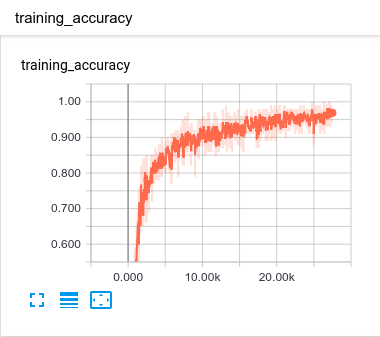
\includegraphics[width=.99\linewidth]{1.png}
  \captionof{}{Training Accuracy Graph}
\end{minipage}%
\begin{minipage}{.5\textwidth}
  \centering
  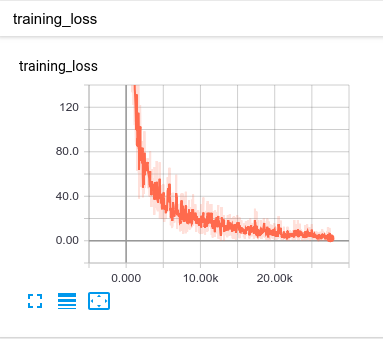
\includegraphics[width=.99\linewidth]{2.png}
  \captionof{}{Training Cost Graph}
\end{minipage}
\end{figure}

\begin{figure}[h]
\centering
\begin{minipage}{.5\textwidth}
  \centering
  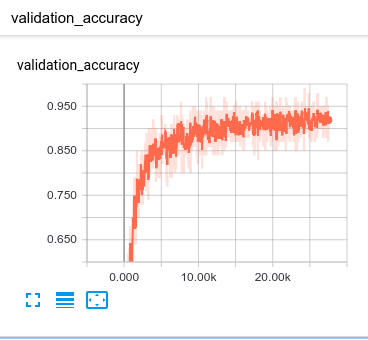
\includegraphics[width=.99\linewidth]{3.png}
  \captionof{}{Validation Accuracy Graph}
\end{minipage}%
\begin{minipage}{.5\textwidth}
  \centering
  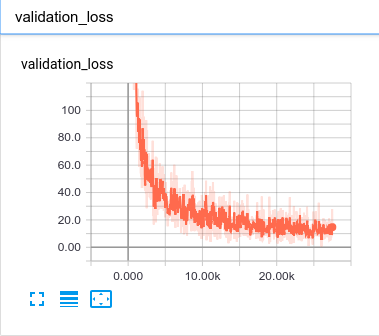
\includegraphics[width=.99\linewidth]{4.png}
  \captionof{}{Validation Cost Graph}
\end{minipage}
\end{figure}
    
\end{document}